%%%%%%%%%%%%%%%%%%%%%%%%%%%%%%%%%%%%%%%%%
% Classicthesis Typographic Thesis
% LaTeX Template
% Version 1.4 (1/1/16)
%
% This template has been downloaded from:
% http://www.LaTeXTemplates.com
%
% Original author:
% André Miede (http://www.miede.de) with commenting modifications by:
% Vel (vel@LaTeXTemplates.com)
%
% License:
% GNU General Public License (v2)
%
% General Tips:
% 1) Make sure to edit the classicthesis-config.file
% 2) New enumeration (A., B., C., etc in small caps): \begin{aenumerate} \end{aenumerate}
% 3) For margin notes: \marginpar or \graffito{}
% 4) Do not use bold fonts in this style, it is designed around them
% 5) Use tables as in the examples
% 6) See classicthesis-preamble.sty for useful commands
%
%%%%%%%%%%%%%%%%%%%%%%%%%%%%%%%%%%%%%%%%%

%----------------------------------------------------------------------------------------
%	PACKAGES AND OTHER DOCUMENT CONFIGURATIONS
%----------------------------------------------------------------------------------------

\documentclass[
		twoside,openright,titlepage,numbers=noenddot,headinclude,%1headlines,
	 	footinclude=true,cleardoublepage=empty,
		dottedtoc, % Make page numbers in the table of contents flushed right with dots leading to them
		BCOR=5mm,paper=a4,fontsize=11pt, % Binding correction, paper type and font size
		ngerman,american, % Languages, change this to your language(s)
		]{scrreprt} 
                
% Includes the file which contains all the document configurations and packages - make sure to edit this file
%%%%%%%%%%%%%%%%%%%%%%%%%%%%%%%%%%%%%%%%%
% Classicthesis Typographic Thesis
% Configuration File
%
% This file has been downloaded from:
% http://www.LaTeXTemplates.com
%
% Original author:
% André Miede (http://www.miede.de) with extensive commenting changes by:
% Vel (vel@LaTeXTemplates.com)
%
% License:
% GNU General Public License (v2)
%
% Important note:
% The main lines to change in this file are in the DOCUMENT VARIABLES
% section, the rest of the file is for advanced configuration.
%
%%%%%%%%%%%%%%%%%%%%%%%%%%%%%%%%%%%%%%%%%

%----------------------------------------------------------------------------------------
%	CHARACTER ENCODING
%----------------------------------------------------------------------------------------

\PassOptionsToPackage{utf8}{inputenc} % Set the encoding of your files. UTF-8 is the only sensible encoding nowadays. If you can't read äöüßáéçèê∂åëæƒÏ€ then change the encoding setting in your editor, not the line below. If your editor does not support utf8 use another editor!
\usepackage{inputenc}

%----------------------------------------------------------------------------------------
%	DOCUMENT VARIABLES
%	Fill in the lines below to enter your information into the thesis template
%	Each of the commands can be cited anywhere in the thesis
%----------------------------------------------------------------------------------------

% Remove drafting to get rid of the '[ Date - classicthesis version 4.0 ]' text at the bottom of every page
\PassOptionsToPackage{eulerchapternumbers,listings,drafting, pdfspacing, subfig,beramono,eulermath,parts}{classicthesis}
% Available options: drafting parts nochapters linedheaders eulerchapternumbers beramono eulermath pdfspacing minionprospacing tocaligned dottedtoc manychapters listings floatperchapter subfig

\newcommand{\myTitle}{A Search for Supersymmetry in Events with a Z Boson, Jets, and Missing Transverse Energy in $p-p$ Collisions with $\sqrt{s}$=13 TeV with the ATLAS Detector\xspace}
\newcommand{\mySubtitle}{ ?? \xspace}
\newcommand{\myDegree}{Doctor of Philosophy (PhD)\xspace}
\newcommand{\myName}{Tova Ray Holmes\xspace}
\newcommand{\myProf}{Dr. Beate Heinemann\xspace}
\newcommand{\myOtherProf}{Put name here\xspace}
\newcommand{\mySupervisor}{Put name here\xspace}
\newcommand{\myFaculty}{Put data here\xspace}
\newcommand{\myDepartment}{Physics Department\xspace}
\newcommand{\myUni}{University of California, Berkeley\xspace}
\newcommand{\myLocation}{Berkeley, CA\xspace}
\newcommand{\myTime}{August 2016\xspace}
\newcommand{\myVersion}{version 1.0\xspace}

%----------------------------------------------------------------------------------------
%	USEFUL COMMANDS
%----------------------------------------------------------------------------------------

\newcommand{\ie}{i.\,e.}
\newcommand{\Ie}{I.\,e.}
\newcommand{\eg}{e.\,g.}
\newcommand{\Eg}{E.\,g.} 

\newcounter{dummy} % Necessary for correct hyperlinks (to index, bib, etc.)
\providecommand{\mLyX}{L\kern-.1667em\lower.25em\hbox{Y}\kern-.125emX\@}
\newlength{\abcd} % for ab..z string length calculation

%----------------------------------------------------------------------------------------
%	PACKAGES
%----------------------------------------------------------------------------------------

\usepackage{lipsum} % Used for inserting dummy 'Lorem ipsum' text into the template
\usepackage{bm} % Used for boldface math 

%------------------------------------------------

%\PassOptionsToPackage{ngerman,american}{babel}  % Change this to your language(s)
% Spanish languages need extra options in order to work with this template
%\PassOptionsToPackage{spanish,es-lcroman}{babel}
\usepackage{babel}

%------------------------------------------------			

\usepackage{csquotes}
\PassOptionsToPackage{%
%backend=biber, % Instead of bibtex
backend=bibtex8,bibencoding=ascii,%
language=auto,%
style=numeric-comp,%
%style=authoryear-comp, % Author 1999, 2010
%bibstyle=authoryear,dashed=false, % dashed: substitute rep. author with ---
sorting=nyt, % name, year, title
maxbibnames=10, % default: 3, et al.
%backref=true,%
natbib=true % natbib compatibility mode (\citep and \citet still work)
}{biblatex}
\usepackage{biblatex}
 
 %------------------------------------------------

\PassOptionsToPackage{fleqn}{amsmath} % Math environments and more by the AMS 
 \usepackage{amsmath}
 
 %------------------------------------------------

\PassOptionsToPackage{T1}{fontenc} % T2A for cyrillics
\usepackage{fontenc}

%------------------------------------------------

\usepackage{textcomp} % Fix warning with missing font shapes

%------------------------------------------------

\usepackage{scrhack} % Fix warnings when using KOMA with listings package  

%------------------------------------------------

\usepackage{xspace} % To get the spacing after macros right

%------------------------------------------------

\usepackage{mparhack} % To get marginpar right

%------------------------------------------------

\usepackage{fixltx2e} % Fixes some LaTeX stuff 

%------------------------------------------------

\PassOptionsToPackage{smaller}{acronym} % Include printonlyused in the first bracket to only show acronyms used in the text
\usepackage{acronym} % Nice macros for handling all acronyms in the thesis

%\renewcommand*{\acsfont}[1]{\textssc{#1}} % For MinionPro
\renewcommand*{\aclabelfont}[1]{\acsfont{#1}}

%------------------------------------------------

\PassOptionsToPackage{pdftex}{graphicx}
\usepackage{graphicx} 

%----------------------------------------------------------------------------------------
%	FLOATS: TABLES, FIGURES AND CAPTIONS SETUP
%----------------------------------------------------------------------------------------

\usepackage{tabularx} % Better tables
\setlength{\extrarowheight}{3pt} % Increase table row height
\newcommand{\tableheadline}[1]{\multicolumn{1}{c}{\spacedlowsmallcaps{#1}}}
\newcommand{\myfloatalign}{\centering} % To be used with each float for alignment
\usepackage{caption}
\captionsetup{font=small}
\usepackage{subfig}  

%----------------------------------------------------------------------------------------
%	CODE LISTINGS SETUP
%----------------------------------------------------------------------------------------

\usepackage{listings} 
%\lstset{emph={trueIndex,root},emphstyle=\color{BlueViolet}}%\underbar} % For special keywords
\lstset{language=[LaTeX]Tex,%C++ % Specify the language(s) for listings here
morekeywords={PassOptionsToPackage,selectlanguage},
keywordstyle=\color{RoyalBlue}, % Add \bfseries for bold
basicstyle=\small\ttfamily, % Makes listings a smaller font size and a different font
%identifierstyle=\color{NavyBlue}, % Color of text inside brackets
commentstyle=\color{Green}\ttfamily, % Color of comments
stringstyle=\rmfamily, % Font type to use for strings
numbers=left, % Change left to none to remove line numbers
numberstyle=\scriptsize, % Font size of the line numbers
stepnumber=5, % Increment of line numbers
numbersep=8pt, % Distance of line numbers from code listing
showstringspaces=false, % Sets whether spaces in strings should appear underlined
breaklines=true, % Force the code to stay in the confines of the listing box
%frameround=ftff, % Uncomment for rounded frame
%frame=single, % Frame border - none/leftline/topline/bottomline/lines/single/shadowbox/L
belowcaptionskip=.75\baselineskip % Space after the "Listing #: Desciption" text and the listing box
}

%----------------------------------------------------------------------------------------
%	HYPERREFERENCES
%----------------------------------------------------------------------------------------

\PassOptionsToPackage{pdftex,hyperfootnotes=false,pdfpagelabels}{hyperref}
\usepackage{hyperref}  % backref linktocpage pagebackref
\pdfcompresslevel=9
\pdfadjustspacing=1

\hypersetup{
% Uncomment the line below to remove all links (to references, figures, tables, etc), useful for b/w printouts
%draft, 
colorlinks=true, linktocpage=true, pdfstartpage=3, pdfstartview=FitV,
% Uncomment the line below if you want to have black links (e.g. for printing black and white)
%colorlinks=false, linktocpage=false, pdfborder={0 0 0}, pdfstartpage=3, pdfstartview=FitV, 
breaklinks=true, pdfpagemode=UseNone, pageanchor=true, pdfpagemode=UseOutlines,%
plainpages=false, bookmarksnumbered, bookmarksopen=true, bookmarksopenlevel=1,%
hypertexnames=true, pdfhighlight=/O,%nesting=true,%frenchlinks,%
urlcolor=RoyalBlue, linkcolor=RoyalBlue, citecolor=webgreen, %pagecolor=RoyalBlue,%
    %urlcolor=Black, linkcolor=Black, citecolor=Black, %pagecolor=Black,%
%------------------------------------------------
% PDF file meta-information
pdftitle={\myTitle},
pdfauthor={\textcopyright\ \myName, \myUni, \myFaculty},
pdfsubject={},
pdfkeywords={},
pdfcreator={pdfLaTeX},
pdfproducer={LaTeX with hyperref and classicthesis}
%------------------------------------------------
}

%----------------------------------------------------------------------------------------
%	AUTOREFERENCES SETUP
%	Redefines how references in text are prefaced for different 
%	languages (e.g. "Section 1.2" or "section 1.2")
%----------------------------------------------------------------------------------------

\makeatletter
\@ifpackageloaded{babel}
{
\addto\extrasamerican{
\renewcommand*{\figureautorefname}{Figure}
\renewcommand*{\tableautorefname}{Table}
\renewcommand*{\partautorefname}{Part}
\renewcommand*{\chapterautorefname}{Chapter}
\renewcommand*{\sectionautorefname}{Section}
\renewcommand*{\subsectionautorefname}{Section}
\renewcommand*{\subsubsectionautorefname}{Section}
}
\addto\extrasngerman{
\renewcommand*{\paragraphautorefname}{Absatz}
\renewcommand*{\subparagraphautorefname}{Unterabsatz}
\renewcommand*{\footnoteautorefname}{Fu\"snote}
\renewcommand*{\FancyVerbLineautorefname}{Zeile}
\renewcommand*{\theoremautorefname}{Theorem}
\renewcommand*{\appendixautorefname}{Anhang}
\renewcommand*{\equationautorefname}{Gleichung}
\renewcommand*{\itemautorefname}{Punkt}
}
\providecommand{\subfigureautorefname}{\figureautorefname} % Fix to getting autorefs for subfigures right
}{\relax}
\makeatother

%----------------------------------------------------------------------------------------

\usepackage{classicthesis} 

%----------------------------------------------------------------------------------------
%	CHANGING TEXT AREA 
%----------------------------------------------------------------------------------------

%\linespread{1.05} % a bit more for Palatino
%\areaset[current]{312pt}{761pt} % 686 (factor 2.2) + 33 head + 42 head \the\footskip
%\setlength{\marginparwidth}{7em}%
%\setlength{\marginparsep}{2em}%

%----------------------------------------------------------------------------------------
%	USING DIFFERENT FONTS
%----------------------------------------------------------------------------------------

%\usepackage[oldstylenums]{kpfonts} % oldstyle notextcomp
%\usepackage[osf]{libertine}
%\usepackage[light,condensed,math]{iwona}
%\renewcommand{\sfdefault}{iwona}
%\usepackage{lmodern} % <-- no osf support :-(
%\usepackage{cfr-lm} % 
%\usepackage[urw-garamond]{mathdesign} <-- no osf support :-(
%\usepackage[default,osfigures]{opensans} % scale=0.95 
%\usepackage[sfdefault]{FiraSans}

\addbibresource{Bibliography.bib} % The file housing your bibliography
%\addbibresource[label=ownpubs]{Self_Publications.bib} % Uncomment for optional self-publications

%\hyphenation{Put special hyphenation here}

\begin{document}

\frenchspacing % Reduces space after periods to make text more compact

\raggedbottom % Makes all pages the height of the text on that page

\selectlanguage{american} % Select your default language - e.g. american or ngerman

%\renewcommand*{\bibname}{new name} % Uncomment to change the name of the bibliography
%\setbibpreamble{} % Uncomment to include a preamble to the bibliography - some text before the reference list starts

\pagenumbering{roman} % Roman page numbering prior to the start of the thesis content (i, ii, iii, etc)

\pagestyle{plain} % Suppress headers for the pre-content pages

%----------------------------------------------------------------------------------------
%	PRE-CONTENT THESIS PAGES
%----------------------------------------------------------------------------------------

% Title Page

\begin{titlepage}

\begin{addmargin}[-1cm]{-3cm}
\begin{center}
\large

\hfill
\vfill

\begingroup
\color{RoyalBlue}\spacedallcaps{\myTitle} \\ \bigskip % Thesis title
\endgroup

\spacedlowsmallcaps{\myName} % Your name

\vfill


\includegraphics[width=5cm]{gfx/ucberkeleyseal_line_540.eps} \\ \medskip % Picture

\mySubtitle \\ \medskip % Thesis subtitle
%\myDegree \\
%\myDepartment \\
%\myFaculty \\
%\myUni \\ \bigskip

\myTime\ -- \myVersion % Time and version

\vfill

\end{center}
\end{addmargin}

\end{titlepage} % Main title page

% Back of the title page

\thispagestyle{empty}

\hfill

\vfill

\noindent\myName: \textit{\myTitle,} %\mySubtitle, %\myDegree, 
\textcopyright\ \myTime

% You may wish to do something with the back of the title page, such as including your supervisors, location or time frame of the work. Below is an example of doing so although you may want to tweak it to your liking.

%\bigskip

%\noindent\spacedlowsmallcaps{Supervisors}: \\
%\myProf \\
%\myOtherProf \\ 
%\mySupervisor

%\medskip \\

%\noindent\spacedlowsmallcaps{Location}: \\
%\myLocation

%\medskip \\

%\noindent\spacedlowsmallcaps{Time Frame}: \\
%\myTime
 % Back of the title page

\cleardoublepage% Dedication

\thispagestyle{empty}
\refstepcounter{dummy}

\pdfbookmark[1]{Dedication}{Dedication} % Bookmark name visible in a PDF viewer

\vspace*{3cm}

\begin{center}
%To my brother for at least starting to lead the way.
\end{center}

%\medskip

%\begin{center}
%Dedicated to the loving memory of Rudolf Miede. \\ \smallskip
%1939\,--\,2005
%\end{center} % Dedication page

%\cleardoublepage\include{FrontBackMatter/Foreword} % Uncomment and create a Foreword.tex to include a foreword

\cleardoublepage% Abstract

%\renewcommand{\abstractname}{Abstract} % Uncomment to change the name of the abstract

\pdfbookmark[1]{Abstract}{Abstract} % Bookmark name visible in a PDF viewer

\begingroup
\let\clearpage\relax
\let\cleardoublepage\relax
\let\cleardoublepage\relax

\chapter*{Abstract}
Short summary of the contents\dots a great guide by 
Kent Beck how to write good abstracts can be found here:  
\begin{center}
\url{https://plg.uwaterloo.ca/~migod/research/beckOOPSLA.html}
\end{center}

\endgroup			

\vfill % Abstract page

\cleardoublepage% Publications - a page listing research articles written using content in the thesis

\pdfbookmark[1]{Publications}{Publications} % Bookmark name visible in a PDF viewer

\chapter*{Publications} % Publications page text

Some ideas and figures have appeared previously in the following publications:\\

\noindent Put your publications from the thesis here. The packages \texttt{multibib} or \texttt{bibtopic} etc. can be used to handle multiple different bibliographies in your document.

%\begin{refsection}[ownpubs]
%    \small
%    \nocite{*} % is local to to the enclosing refsection
%    \printbibliography[heading=none]
%\end{refsection}

%\emph{Attention}: This requires a separate run of \texttt{bibtex} for your \texttt{refsection}, \eg, \texttt{ClassicThesis1-blx} for this file. You might also use \texttt{biber} as the backend for \texttt{biblatex}. See also \url{http://tex.stackexchange.com/questions/128196/problem-with-refsection}. % Publications from the thesis page

\cleardoublepage% Acknowledgements

\pdfbookmark[1]{Acknowledgements}{Acknowledgements} % Bookmark name visible in a PDF viewer



\bigskip

%----------------------------------------------------------------------------------------

\begingroup

\let\clearpage\relax
\let\cleardoublepage\relax
\let\cleardoublepage\relax

\chapter*{Acknowledgements}

\noindent Put your acknowledgements here.\\



\endgroup % Acknowledgements page

\pagestyle{scrheadings} % Show chapter titles as headings

\cleardoublepage% Table of Contents - List of Tables/Figures/Listings and Acronyms

\refstepcounter{dummy}

\pdfbookmark[1]{\contentsname}{tableofcontents} % Bookmark name visible in a PDF viewer

\setcounter{tocdepth}{2} % Depth of sections to include in the table of contents - currently up to subsections

\setcounter{secnumdepth}{3} % Depth of sections to number in the text itself - currently up to subsubsections

\manualmark
\markboth{\spacedlowsmallcaps{\contentsname}}{\spacedlowsmallcaps{\contentsname}}
\tableofcontents 
\automark[section]{chapter}
\renewcommand{\chaptermark}[1]{\markboth{\spacedlowsmallcaps{#1}}{\spacedlowsmallcaps{#1}}}
\renewcommand{\sectionmark}[1]{\markright{\thesection\enspace\spacedlowsmallcaps{#1}}}

\clearpage

\begingroup 
\let\clearpage\relax
\let\cleardoublepage\relax
\let\cleardoublepage\relax

%----------------------------------------------------------------------------------------
%	List of Figures
%----------------------------------------------------------------------------------------

\refstepcounter{dummy}
%\addcontentsline{toc}{chapter}{\listfigurename} % Uncomment if you would like the list of figures to appear in the table of contents
\pdfbookmark[1]{\listfigurename}{lof} % Bookmark name visible in a PDF viewer

\renewcommand{\sectionmark}[1]{\markright{\thesection\enspace\spacedlowsmallcaps{#1}}} 
\listoffigures

\vspace{8ex}
\newpage

%----------------------------------------------------------------------------------------
%	List of Tables
%----------------------------------------------------------------------------------------

\refstepcounter{dummy}
%\addcontentsline{toc}{chapter}{\listtablename} % Uncomment if you would like the list of tables to appear in the table of contents
\pdfbookmark[1]{\listtablename}{lot} % Bookmark name visible in a PDF viewer

\listoftables
        
\vspace{8ex}
\newpage
    
%----------------------------------------------------------------------------------------
%	List of Listings
%---------------------------------------------------------------------------------------- 

%\refstepcounter{dummy}
%\addcontentsline{toc}{chapter}{\lstlistlistingname} % Uncomment if you would like the list of listings to appear in the table of contents
%\pdfbookmark[1]{\lstlistlistingname}{lol} % Bookmark name visible in a PDF viewer

%\lstlistoflistings 

%\vspace{8ex}
%\newpage
       
%----------------------------------------------------------------------------------------
%	Acronyms
%----------------------------------------------------------------------------------------

\refstepcounter{dummy}
%\addcontentsline{toc}{chapter}{Acronyms} % Uncomment if you would like the acronyms to appear in the table of contents
\pdfbookmark[1]{Acronyms}{acronyms} % Bookmark name visible in a PDF viewer

\markboth{\spacedlowsmallcaps{Acronyms}}{\spacedlowsmallcaps{Acronyms}}

\chapter*{Acronyms}

\begin{acronym}[UML]
% detector acronyms
\acro{IBL}{Insertable B-Layer}
\acro{MS}{Muon Spectrometer}
\acro{ID}{Inner Detector}
\acro{SCT}{Silicon Microstrip Tracker}
\acro{TRT}{Transition Radiation Tracker}
\acro{NN}{Neural Network}
\acro{CCA}{Connected Component Analysis}
\acro{ToT}{Time Over Threshold}
\acro{MDT}{Monitored Drift Tube}
\acro{CSC}{Cathode-Strip Chamber}
\acro{RPC}{Resistive Plate Chamber}
\acro{TGC}{Thin Gap Chamber}
\acro{L1}{Level One}
\acro{HLT}{High Level Trigger}
\acro{L1Calo}{L1 Calorimeter Trigger}
\acro{L1Topo}{L1 Topological Trigger}
\acro{CTP}{Central Trigger Processor}
\acro{TTC}{Trigger Timing and Control}
\acro{ROB}{Read Out Board}
\acro{RoI}{Region of Interest}
%lhc acronyms
\acro{LHC}{Large Hadron Collider}
\acro{LEP}{Large Electron-Positron}
\acro{SPS}{Super Proton Synchrotron}
\acro{ATLAS}{A Toroidal LHC Apparatus}
\acro{CMS}{Compact Muon Solenoid}
\acro{ALICE}{A Large Ion Collider Experiment}
\acro{LHCb}{Large Hadron Collider beauty}
\acro{RF}{Radiofrequency}
\acro{PSB}{Proton Synchrotron Booster}
\acro{PS}{Proton Synchrotron}
% reco acronyms
\acro{OR}{Overlap Removal}
\acro{EM}{Electromagnetic}
\acro{LCW}{Local Cluster Weighting}
\acro{JES}{Jet Energy Scale}
\acro{JER}{Jet Energy Resolution}
\acro{JVT}{Jet Vertex Tagger}
\acro{JVF}{Jet Vertex Fraction}
\acro{CST}{Calorimeter Soft Term}
\acro{TST}{Track Soft Term}

% theory acronyms
\acro{MC}{Monte Carlo simulation}
\acro{SM}{Standard Model}
\acro{BSM}{Beyond the Standard Model}
\acro{SUSY}{Supersymmetry}
\acro{QCD}{Quantum Chromodynamics}
\acro{PDF}{Parton Distribution Function}
\acro{DM}{Dark Matter}
\acro{LO}{Leading Order}
\acro{NLO}{Next to Leading Order}
\acro{NLO+NLL}{Next-to-Leading-Logarithmic Accuracy}
\acro{SUSY}{Supersymmetry}
\acro{MSSM}{Minimal Supersymmetric Standard Model}
\acro{LSP}{Lightest Supersymmetric Particle}
% analysis acronyms
\acro{AOD}{Analysis Object Data}
\acro{dAOD}{derived AOD}
\acro{SR}{Signal Region}
\acro{VR}{Validation Region}
\acro{CR}{Control Region}
\acro{FS}{Flavor Symmetric}
\acro{CL}{Confidence Level}
\acro{HL-LHC}{High Luminosity Large Hadron Collider}
\end{acronym}  
                   
\endgroup % Contents, list of figures/tables/listings and acronyms

\cleardoublepage

\pagenumbering{arabic} % Arabic page numbering for thesis content (1, 2, 3, etc)
%\setcounter{page}{90} % Uncomment to manually start the page counter at an arbitrary value (for example if you wish to count the pre-content pages in the page count)

\cleardoublepage % Avoids problems with pdfbookmark

%----------------------------------------------------------------------------------------
%	THESIS CONTENT - CHAPTERS
%----------------------------------------------------------------------------------------

\ctparttext{You can put some informational part preamble text here. Illo principalmente su nos. Non message \emph{occidental} angloromanic da. Debitas effortio simplificate sia se, auxiliar summarios da que, se avantiate publicationes via. Pan in terra summarios, capital interlingua se que. Al via multo esser specimen, campo responder que da. Le usate medical addresses pro, europa origine sanctificate nos se.} % Text on the Part 1 page describing  the content in Part 1

\part{Some Kind of Manual} % First part of the thesis

% Chapter 1

\chapter{Introduction} % Chapter title

\label{ch:introduction} % For referencing the chapter elsewhere, use \autoref{ch:introduction} 

%----------------------------------------------------------------------------------------

In 2010, the \acf{LHC} began colliding high energy protons in its 27 km ring, taking its place as the most powerful in a long line of accelerators aimed at uncovering the fundamental rules that govern particle physics. Its primary goal was to complete the Standard Model of particle physics by discovering the Higgs boson, the last remaining particle that was predicted by this model but not yet observed. With its presence, the Standard Model would be consistent, explaining every observed interaction of known particles, with a complete mathematic framework to describe each feature. However, even with a Higgs boson, the Standard Model contained hints that it might be incomplete, suspicious features that suggested that at a higher energy, there might be something more.

In 2012, the \acs{ATLAS} (\aclu{ATLAS}) and \acs{CMS} (\aclu{CMS}) Experiments discovered the Higgs boson, leaving the \ac{LHC} physics community without a single primary goal, but rather a host of theories to explore, each extending the Standard Model in a different way. Each theory attempts to solve one of the mysteries left by the Standard Model, providing an explanation for Dark Matter, suggesting a mechanism that could explain gravity's weakness, or explaining the Higgs boson's mass value. For decades, the most popular of these has been Supersymmetry, which proposes a fermionic symmetry and requires a menagerie of new Supersymmetric particles, none of which has yet been observed. 

Supersymmetry simultaneously solves more of the Standard Mo\-del's problems than any other theory, making it appealing to theorists and experimentalists alike. But in order to do this, Supersymmetric particles must appear with masses of approximately 1 \tev, precisely the range of energies the \ac{LHC} is capable of exploring. In 2015, after a three-year shutdown, the \ac{LHC} nearly doubled the center-of-mass energy of its collisions. This opened up new territory to be explored by analyzers, and provided data that could be used to either discover or exclude many Supersymmetric models.

The analysis presented in this thesis searches for Supersymmetry, seeking to find events in which Supersymmetric particles are produced in proton-proton collisions, then decay via a $Z$ boson to a chargeless Supersymmetric particle which escapes \ac{ATLAS} without detection. A similar \ac{ATLAS} search, performed with data from the lower-energy collisions 2012, observed a $3\sigma$ excess of events over the expected Standard Model background \cite{SUSY-2014-10}. 

The excess generated interest in this channel, and re-investigating it became a top priority when the upgraded \ac{LHC} turned on in 2015. %A preliminary search, performed using 2015 data only, was released at the end of that year. Again an excess was observed, this time with a significance of $2.2\sigma$ \cite{ATLAS-CONF-2015-082}. 

This thesis describes a search for Supersymmetry performed in this channel using data taken by the \ac{ATLAS} detector in 2015 and 2016, including an explanation of the theory and motivation behind the search, and a description of the \ac{LHC} and the \ac{ATLAS} detector. The remaining chapters are laid out as follows: 

\paragraph{Chapter 2} outlines the Standard Model of Particle Physics and the benefits of extending it to include Supersymmetry, then continues on to introduce the specific models used in the search presented in later chapters. 

\paragraph{Chapter 3} describes the \ac{LHC} and its operation, including the magnet system, the preaccelerator complex, and the phenomenology of proton-proton collisions at 13 \tev.

\paragraph{Chapter 4} contains descriptions of the many components of the \ac{ATLAS} detector, and how they serve to detect particles coming from \ac{LHC} collisions. \ac{ATLAS}'s magnet and trigger systems are also discussed. This chapter also provides an overview of the process of generating \ac{MC} for use in the \ac{ATLAS} experiment.

\paragraph{Chapter 5} discusses the tracking system in the \ac{ATLAS} detector, which forms patterns corresponding to particle trajectories out of the many energy deposits left in the detector. This chapter focuses on a neural network designed to improve tracking in the \ac{ATLAS} Pixel Detector, and describes the benefits of its implementation. 

\paragraph{Chapter 6} details the rest of the process of reconstruction, the procedure by which the signals in the \ac{ATLAS} detector are interpreted as particles to be used for analysis. 

\paragraph{Chapter 7} lists the main backgrounds for the Supersymmetry search described in this thesis, and provides general ideas of how they can be reduced. 

\paragraph{Chapter 8} outlines how objects are identified and selected for this analysis, referencing many of the working points defined in Chapter 6.  

\paragraph{Chapter 9} explains the analysis's search strategy, defining signal, control, and validation regions, and briefly describing how each is used in the search.

\paragraph{Chapter 10} describes how estimates of the Standard Model contributions to the signal region are performed for each of the backgrounds listed in Chapter 7. 

\paragraph{Chapter 11} builds off of Chapter 10, and continues to detail how the uncertainties on each estimate are assessed. 

\paragraph{Chapter 12} shows the results of the analysis, comparing expectations based on background estimates to the observed data. 

\paragraph{Chapter 13} provides interpretations of the results, and explains the statistical procedure used to define exclusions on Supersymmetric particles within the models described in Chapter 2. 

\paragraph{Chapter 14} concludes with a summary of the results, and an outlook for future searches. 
 % Chapter 1

\cleardoublepage % Empty page before the start of the next part

%------------------------------------------------

\ctparttext{You can put some informational part preamble text here. Illo principalmente su nos. Non message \emph{occidental} angloromanic da. Debitas effortio simplificate sia se, auxiliar summarios da que, se avantiate publicationes via. Pan in terra summarios, capital interlingua se que. Al via multo esser specimen, campo responder que da. Le usate medical addresses pro, europa origine sanctificate nos se.} % Text on the Part 2 page describing the content in Part 2

\part{The Showcase} % Second part of the thesis

% Chapter 2

\chapter{Theory and Motivation} % Chapter title

\label{ch:theory} % For referencing the chapter elsewhere, use \autoref{ch:examples} 

%----------------------------------------------------------------------------------------

Some kind of preamble here I guess.

%----------------------------------------------------------------------------------------

\section{The Standard Model}

%------------------------------------------------

\subsection{Standard Model Phenomenology}

I will put this off for now.

\subsection{Problems in the Standard Model}

\subsection{Phenomenology of Proton-Proton Collisions}
\subsubsection{Parton Distribution Functions}

%------------------------------------------------

\section{Supersymmetry}

\subsection{Supersymmetry Phenomenology}
\subsection{Solutions to Standard Model Problems}
\subsection{Supersymmetry Signatures in $p-p$ Collisions}
\subsubsection{Simplified Models Used in This Analysis}
\label{sec:simplified_models}

\section{Monte Carlo Generators}
 % Chapter 2
% Chapter 3

\chapter{The Large Hadron Collider} % Chapter title

\label{ch:lhc} % For referencing the chapter elsewhere, use \autoref{ch:mathtest}

%----------------------------------------------------------------------------------------

The \ac{LHC} is unique in the world, producing proton-proton collisions at energies an order of magnitude higher than any accelerator before \cite{1748-0221-3-08-S08001}. It provides unique environments at its collision points where massive, unstable particles can exist for an instant, then decay to the ordinary material of the universe. It is the goal of the ATLAS experiment to identify these short-lived particles, but the \ac{LHC}'s work of producing them is equally complex. 

The \ac{LHC} sits in a 26.7 km circular tunnel that straddles the French-Swiss border outside of Geneva, originally built in 1989 for the \ac{LEP} collider \cite{lep_tdr}. In the \ac{LHC}, two beams of protons are accelerated to 6.5 \tev, then focused and collided at four points around the ring, which can be seen in \autoref{fig:lhc_map}. These points are each encased by particle detectors, which can examine the outputs of the collisions, and have different strengths and goals. The two multipurpose detectors are ATLAS and \ac{CMS}, which have very complex detectors aimed and measuring as many \ac{SM} particles as possible and discovering new processes \cite{PERF-2007-01, 1748-0221-3-08-S08004}. \ac{LHCb} examines processes related to the $b$ quark \cite{1748-0221-3-08-S08005}. Meanwhile, \ac{ALICE} focuses on special runs of the \ac{LHC} which collide lead ions instead of protons, and seeks to understand the high energy densities resulting from the collisions of such massive, complex particles \cite{1748-0221-3-08-S08002}. 

\begin{centering}
\begin{figure}[!hbt]
\myfloatalign
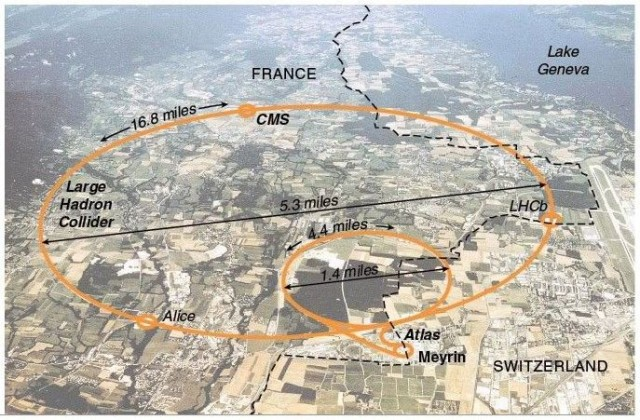
\includegraphics[width=.90\linewidth]{figures/lhc/lhc-5-640x420.jpg}
\caption{The \ac{LHC} main collider ring and pre-accelerator \ac{SPS} overlaid on a map of Switzerland and France, with the four main \ac{LHC} experiments identified.}
\label{fig:lhc_map}
\end{figure}
\end{centering}

%----------------------------------------------------------------------------------------

\section{The Injector Complex}

The goal of the \ac{LHC} is to provide high luminosity proton-proton collisions at 13 \tev. To achieve this, it must be capable of rapidly accelerating large numbers of protons and holding them at a constant energy, and organizing them into bunches which can be focused and collided at precise points and times. To do this, a complex system of pre-accelerators is required, as well as a precisely engineered sytem of magnets within the \ac{LHC}. The full system of pre-accelerators is shown in \autoref{fig:preacc}.

\begin{centering}
\begin{figure}[!hbt]
\myfloatalign
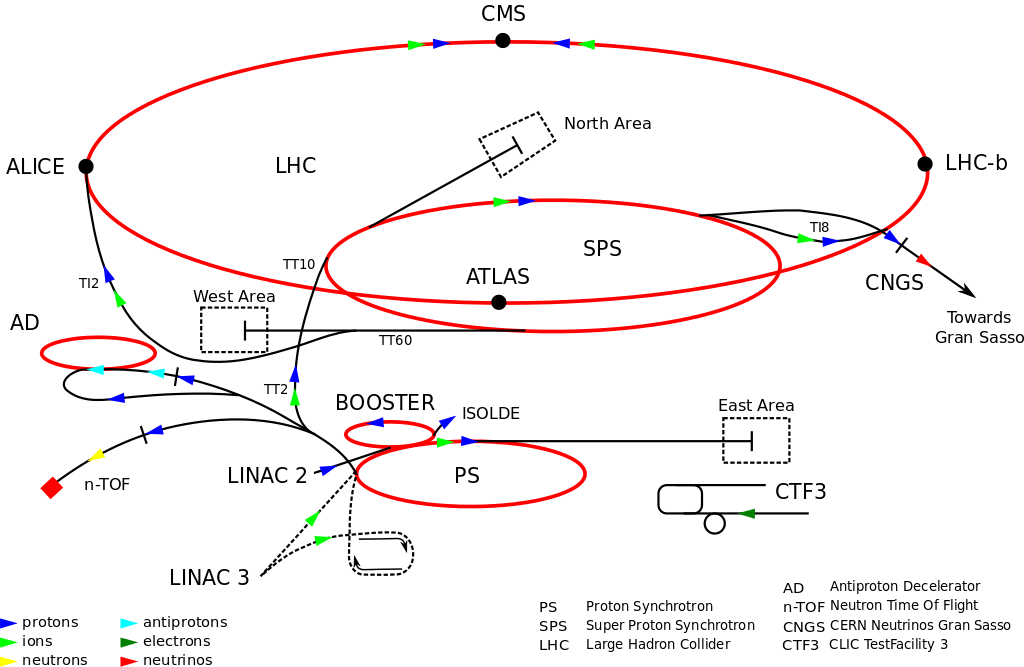
\includegraphics[width=.90\linewidth]{figures/lhc/Cern-accelerator-complex.png}
\caption{The pre-accelerators of the \ac{LHC}.}
\label{fig:preacc}
\end{figure}
\end{centering}

The chain begins with when hydrogen gas is stripped of its electrons and injected in short pulses into Linac2, a linear accelerator which uses \ac{RF} cavities, which use alternating positive and negative electric fields to simultaneously push and pull particles forward through the accelerator. This \ac{RF} behavoir keeps the bunches of protons resulting from the original pulses separated, beginning the formation of the bunch structure used for collisions. Quadropole magnets along the accelerator keep the beam focused. By the end of the accelerator, protons have reached 50 \mev. 

The proton beam is then injected into the \ac{PSB}, the first circular accelerator in the pre-accelerator chain. It increases its magnetic field as the protons increase in speed, ultimately accelerating them to 1.4 \gev. 

At this point the proton beam moves on to the \ac{PS}, a 600 m long circular accelerator that consists of 277 electromagnets that accelerate the protons up to 25 \gev, and 100 additional dipole magnets to bend the beam. 

The last accelerator before injection into the \ac{LHC} is the \ac{SPS}, a 7 km long ring which, long before the \ac{LHC} tunnel was built, was responsible for the discovery of the $W$ and $Z$ bosons. The \ac{SPS} accelerates particles up to 450 \gev~before they are launched into the \ac{LHC}. 

Proton bunches are structured for ease of acceleration, with distinct features resulting from each of the pre-accelerators. The \ac{PS} produces 72 bunches separated by 25 ns, which are injected into the \ac{SPS}, as seen in \autoref{fig:bunches}. However, as the magnetic field directing these protons out of the \ac{PS} loop is turned on, there must be a gap in the bunch structure. Without this gap, called the injection kicker rise time, the changing magnetic field would direct particles out of the accelerator and produce high amounts of unsafe radiation around the \ac{PS}. A similar gap in bunch structure is required for the injection from the \ac{SPS} to the \ac{LHC}. The injection process is repeated until the \ac{LHC} is completely filled with around 2000 bunches, which takes about three minutes.

\begin{centering}
\begin{figure}[!hbt]
\myfloatalign
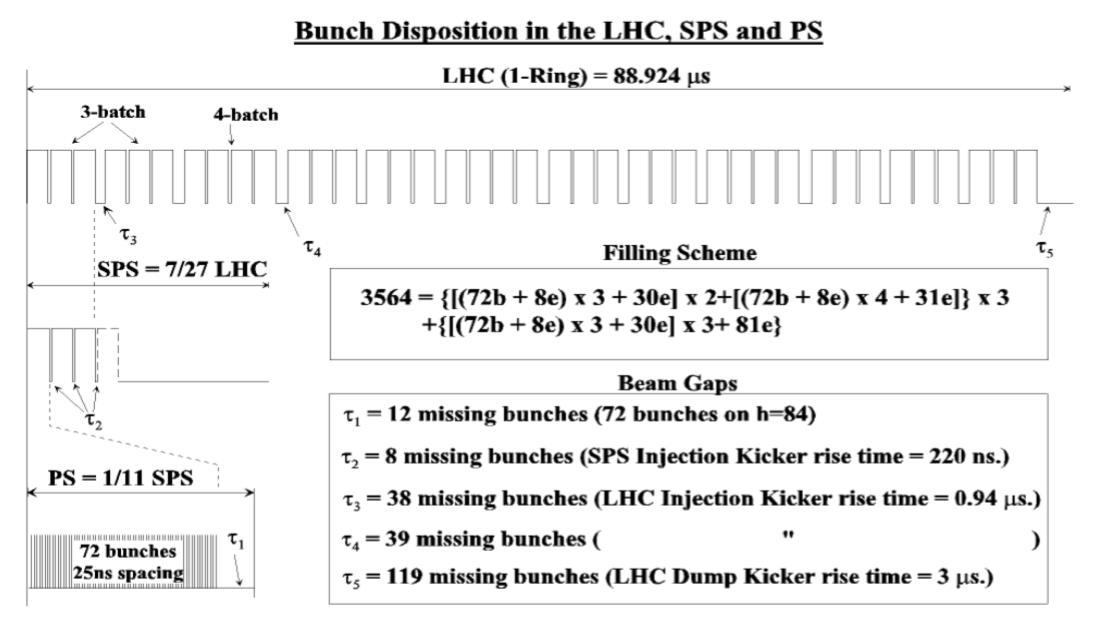
\includegraphics[width=.90\linewidth]{figures/lhc/bunch_structure.png}
\caption{Bunch structure in the \ac{PS}, \ac{SPS}, and \ac{LHC}.}
\label{fig:bunches}
\end{figure}
\end{centering}

\section{Operation of the Large Hadron Collider}

The \ac{LHC} consists of eight straight sections each connected by an arc. In each straigh section, \ac{RF} cavities accelerate protons, ultimately bringing them up to 6.5 \gev. Between these straight sections, 8.4 T dipole magnets bend the beams to maintain the approximately circular path. However, because the \ac{LHC} is a proton-proton collider as opposed to a proton-antiproton collider, the two counter-rotating beams must be housed in separate rings and be accelerated separately. To achieve this, twin-bore superconduncting magnets, one example of which can be seen in \autoref{fig:magnet}, surround the two rings and accelerate them both. Quadropole magnets are used at the four collision points to focus the beams, which cross at an interaction point at the center of a detector. In total there are 1232  main dipole magnets over 5000 additional magnets, which are all are superconducting and kept below their critical temperatures by liquid helium cooling. 

\begin{centering}
\begin{figure}[!hbt]
\myfloatalign
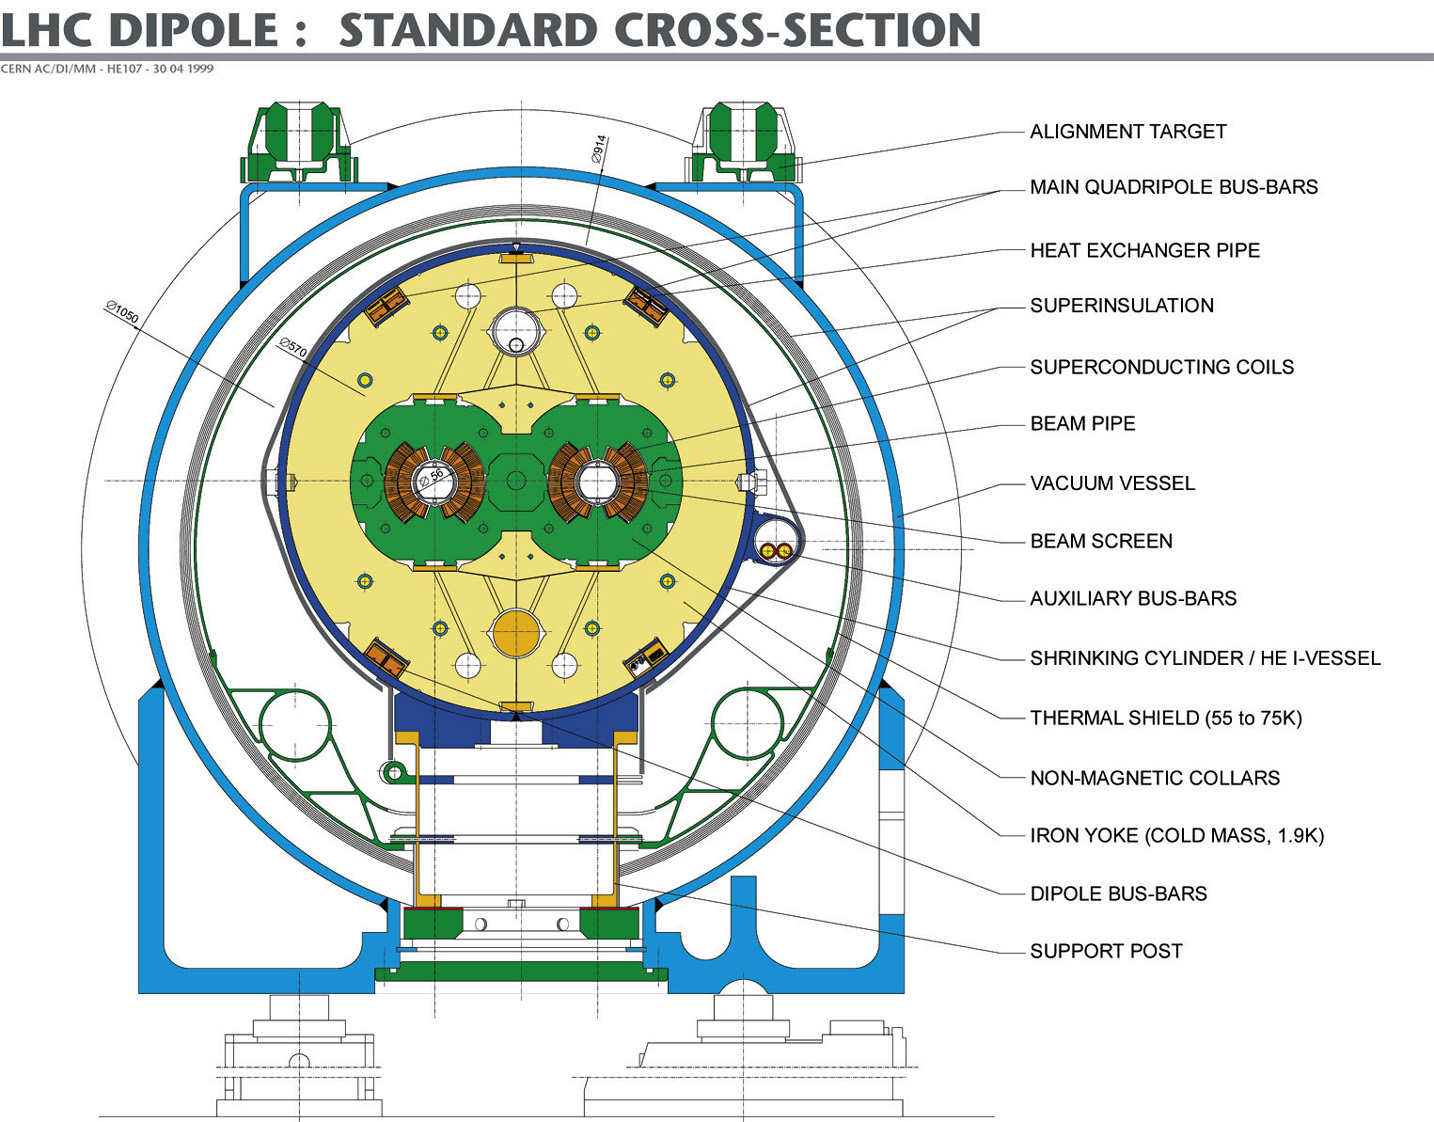
\includegraphics[width=.90\linewidth]{figures/lhc/magnet.jpg}
\caption{Cross-section of a cryodipole magnet in the \ac{LHC}.}
\label{fig:magnet}
\end{figure}
\end{centering}

When first injected into the \ac{LHC}, the protons must be accelerated over many turns through the machine, with the magentic field from the dipoles increasing with each pass to apply more force with which to bend the beam. Once the protons have reached a maximum energy, a process called ``squeezing'' occurs, in which the the total transverse area of the beam is reduced and bunches are elongated slightly. The shape produced by this process determines the ``beam spot'' for the ATLAS detector, the measurement of the area in which collisions occur within the detector. As shown in \autoref{fig:beam_spot}, the collisions all occur very close together in the $x-y$ plane, but have a long spread in the $z$ direction\footnote{The coordinate system used here is discussed in \autoref{sec:coords}.}.

\begin{centering}
\begin{figure}[!hbt]
\myfloatalign
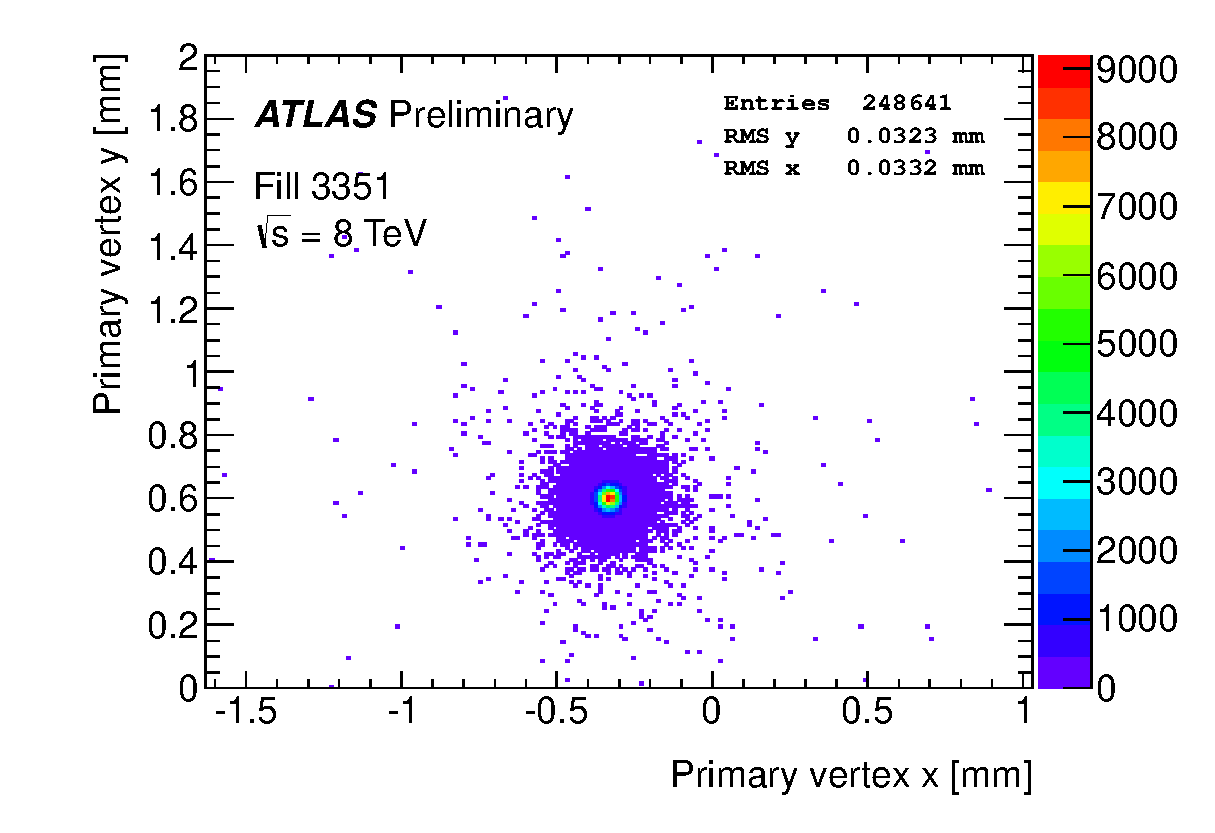
\includegraphics[width=.45\linewidth]{figures/lhc/beamspot-run215456-vtx-yx.eps}
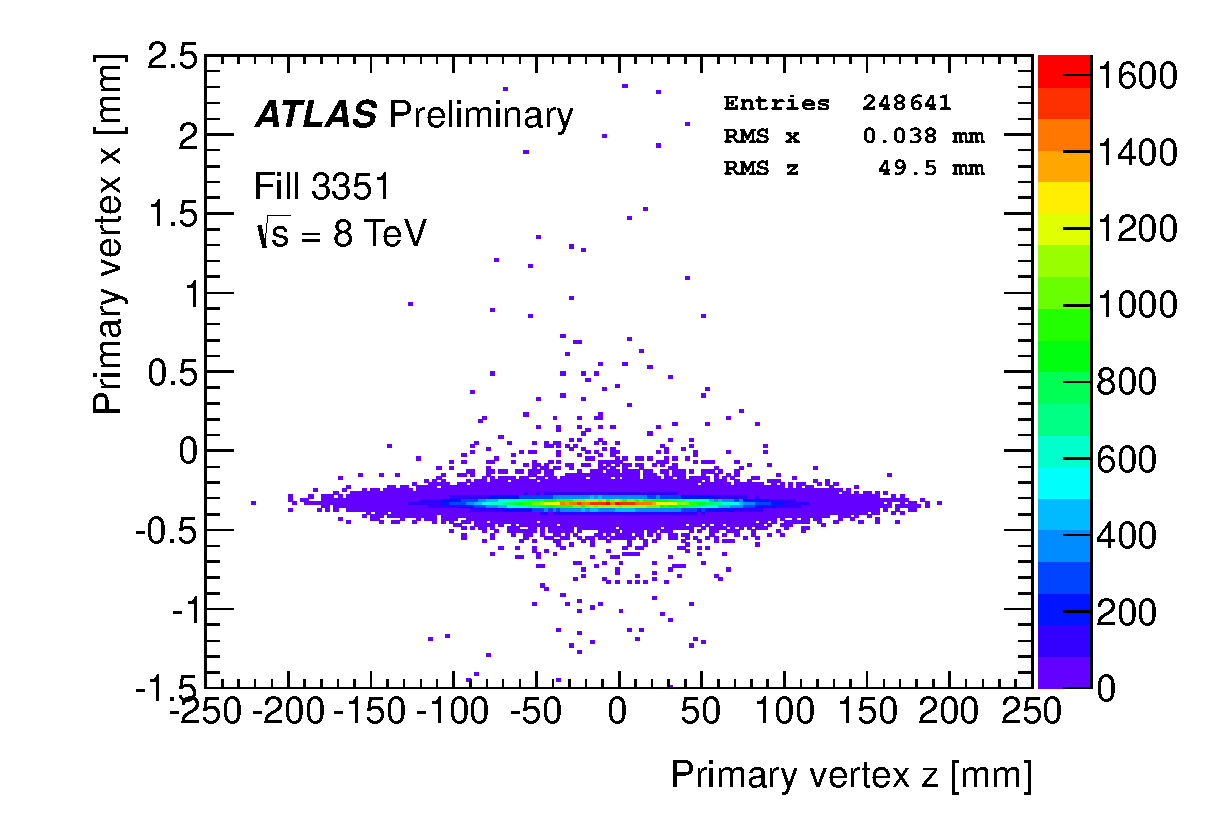
\includegraphics[width=.45\linewidth]{figures/lhc/beamspot-run215456-vtx-xz.eps}
\caption{Beam spot in the ATLAS detector for one run in 2015. Distributions show only the highest \pt vertex per event. Left is the $x-y$ distribution of vertices, while the right plot shows the $x-z$ distribution.}
\label{fig:beam_spot}
\end{figure}
\end{centering}

Once the beams are at a stable energy and have been squeezed, the \ac{LHC} indicates that it is physics-ready to the experiments around the ring, and, after some additional checks by each experiment, data-taking can begin. As collisons occur, the beam is depleted, and when it is sufficiently depleted to require a new fill, or if any instability occurs, the beam is dumped into a cavern filled with steel and concrete, which absorbs the energy. 

\section{Luminosity}

The goal of the collisions provided by the \ac{LHC} is to produce \ac{SM} and \ac{BSM} particles, which can be observed by the detectors. How frequently a given process could occur was a crucial consideration in its design. The number of events of a given type is given by

\begin{equation}
N_{event} = L\sigma_{event}
\end{equation}

where $L$ is the luminosity delivered by the \ac{LHC} and $\sigma_{event}$ is the cross-section of the process in question. These cross-sections vary over many orders of magnitude for different processes, as shown in \autoref{fig:cross_sections}, a plot of many different \ac{SM} cross-sections. As a consequence, a very large amount of luminosity is required to produce the more rare events, and to have enough statistical power to differentiate them from other much more common events.   

\begin{centering}
\begin{figure}[!hbt]
\myfloatalign
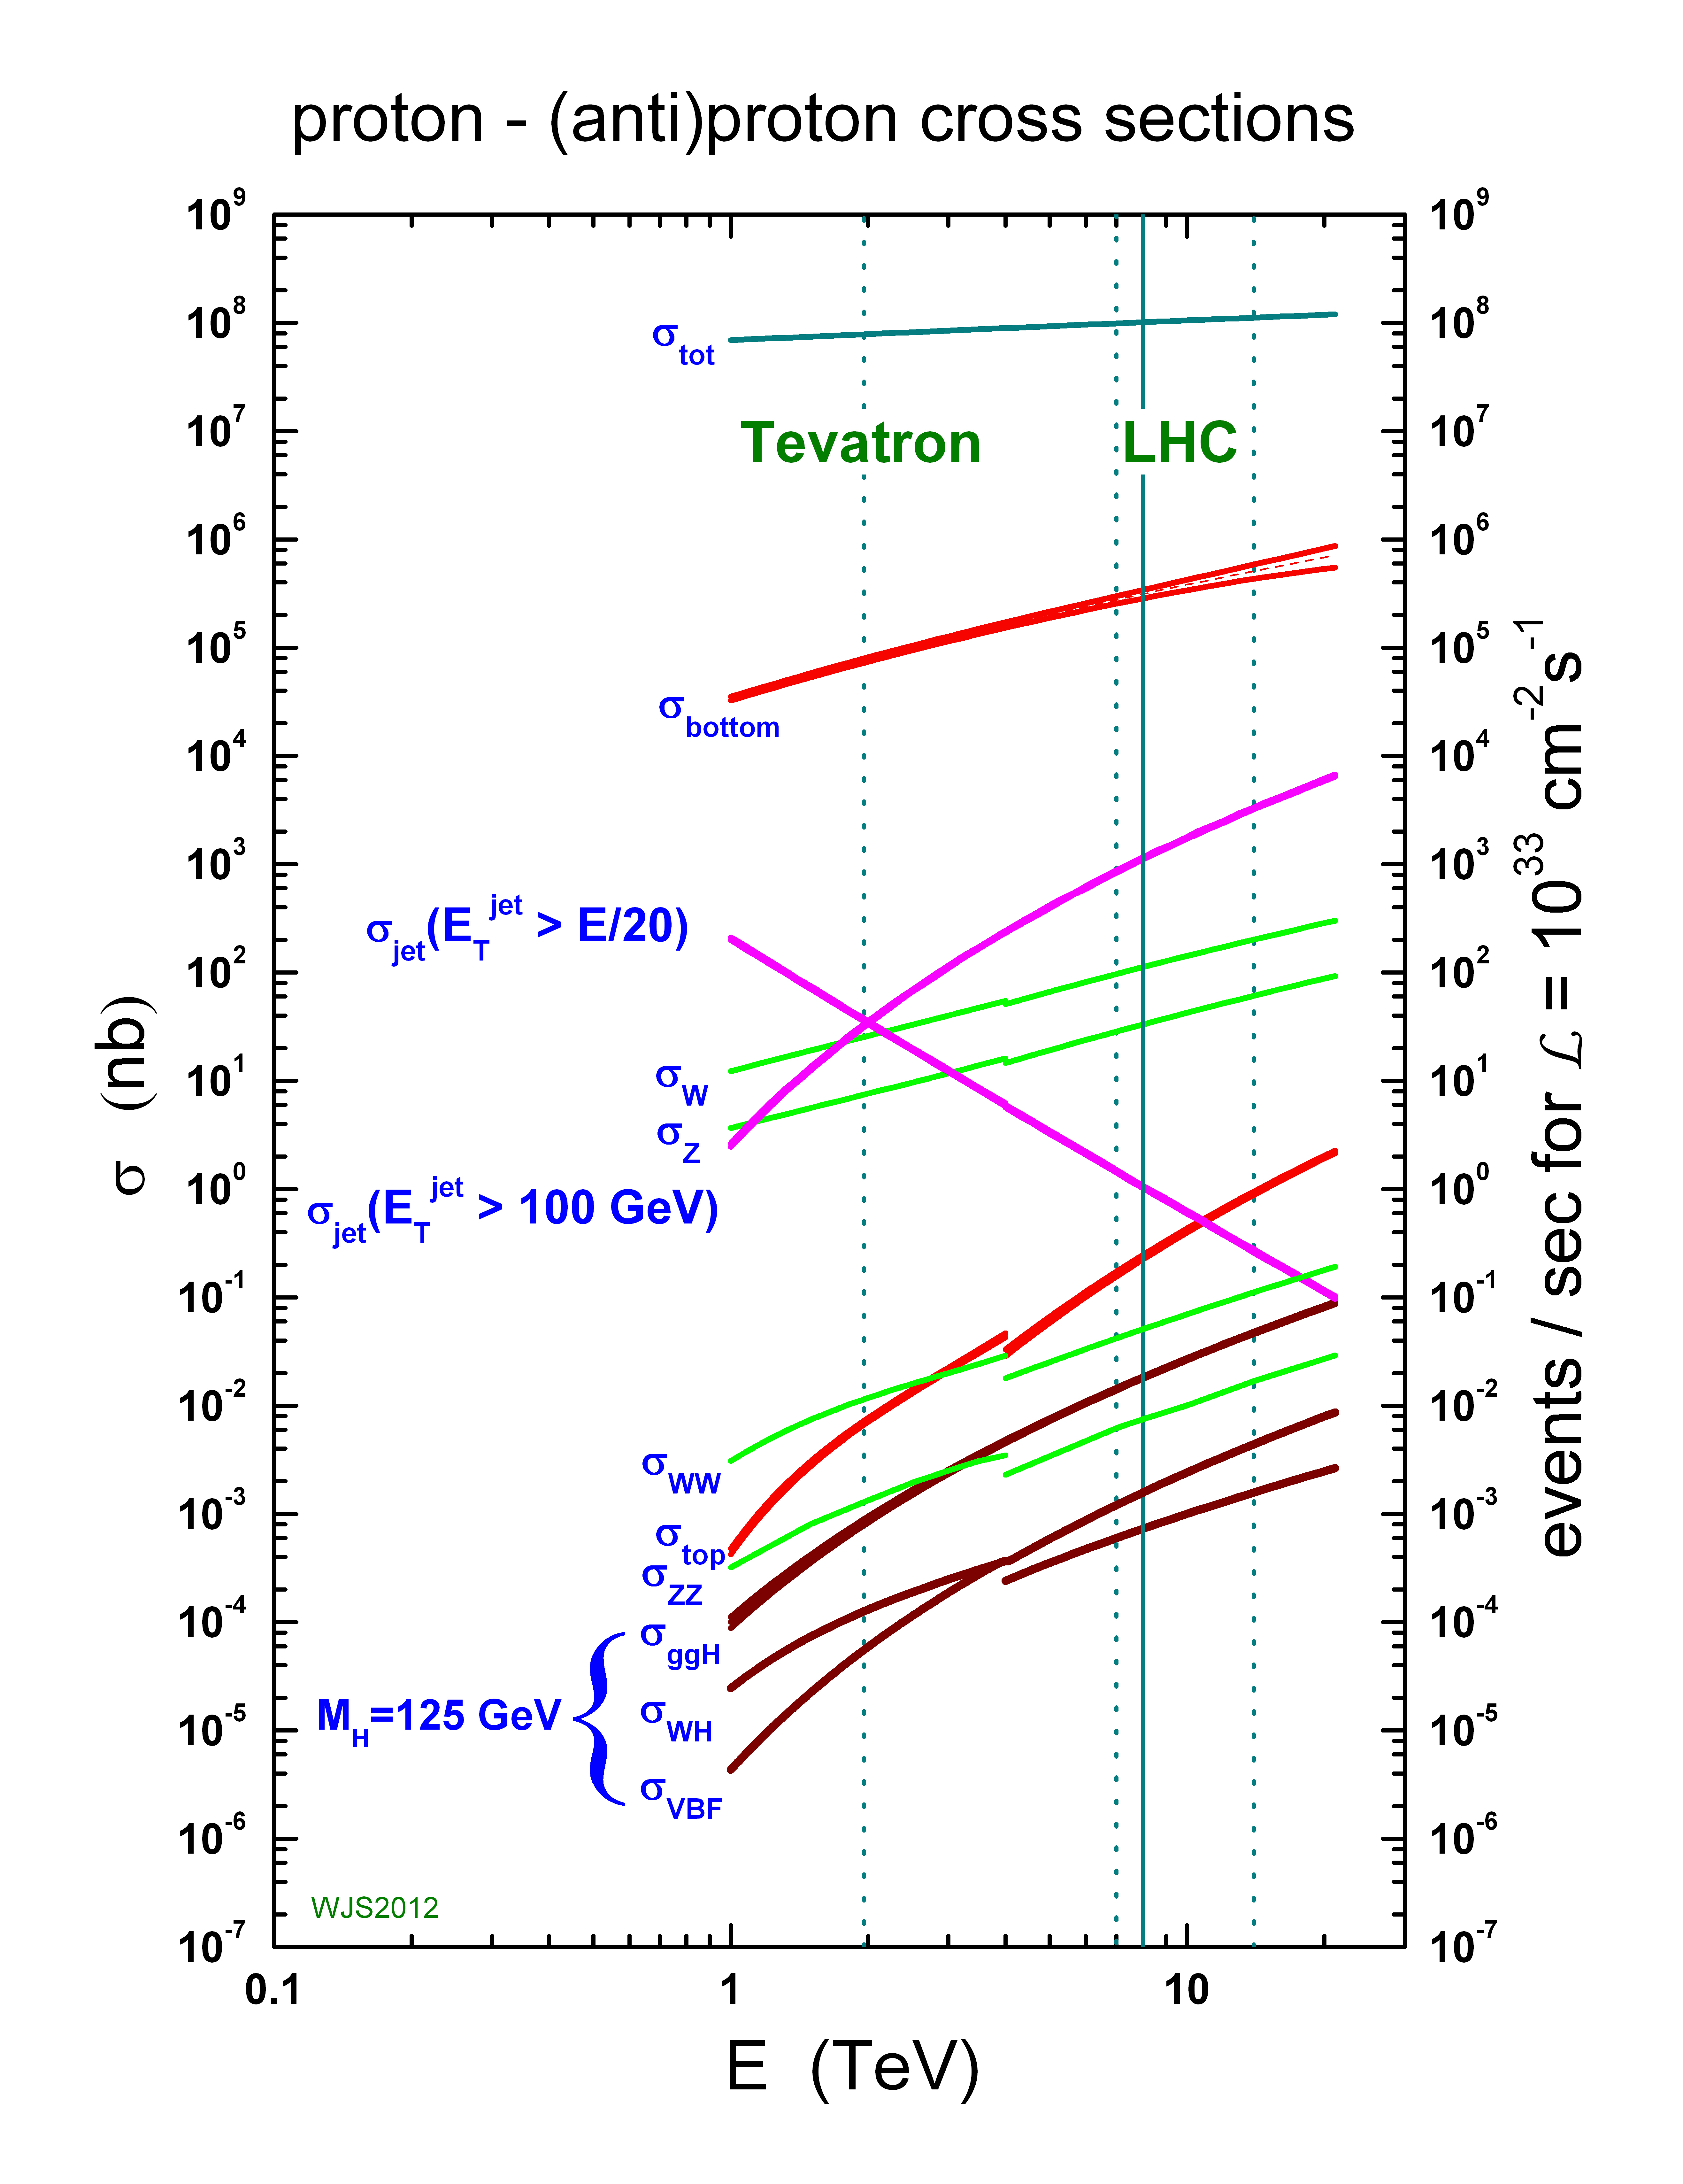
\includegraphics[width=.60\linewidth]{figures/lhc/crosssections2013.jpg}
\caption{Cross-sections for many \ac{SM} processes at the Tevatron and \ac{LHC} \cite{crosssections}.}
\label{fig:cross_sections}
\end{figure}
\end{centering}

The instantaneous luminosity at the \ac{LHC} is given by

\begin{equation}
L = \frac{ N^2_b n_b f_{rev} \gamma_r }{ 4\pi \epsilon_n \beta* } F
\end{equation}

where $N_b$ is the number of protons per bunch ($\sim10^{11}$), $n_b$ is the number of bunches in each beam ($\sim10^3$), $f_{rev}$ is the number of times per second that the beam travels around the ring, $\gamma_r$ is the relativistic gamma factor, $\epsilon_n$ is the normalized transverse beam emittance, and $\beta*$ is the $\beta$-function at the collision point, which describes the transverse displacement of particles in the beam. $F$ gives the reduction factor due to the geometry of the beam crossings, and is given by

\begin{equation}
F = (1+ (\frac{\theta_c \sigma_z}{2\sigma*})^2)^{-1/2}
\end{equation}

where $\theta_c$ is the crossing angle of the beams, $\sigma_z$ is the RMS of the bunch length in the $z$ direction, and $\sigma*$ is the same in the transverse direction.

As the proton beams circulate and collide, $N_b$ decreases, producing a falling instantaneous luminosity, as seen in a Run 1 example in \autoref{fig:instlumi}. In Run 2, peak instantaneous luminosity was brought up to $10^{34}$ cm$^{-2}$s$^{-1}$. This high instantaneous luminosity and consistent running resulted in much faster data collection than in Run 1, which is depicted in \autoref{fig:lumi_vs_year}. 

\begin{centering}
\begin{figure}[!hbt]
\myfloatalign
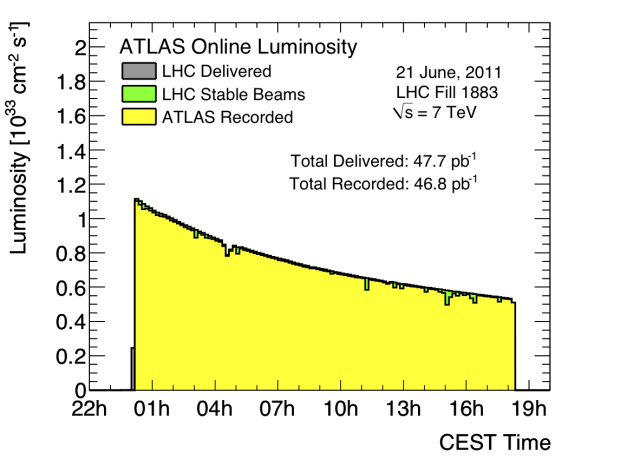
\includegraphics[width=.90\linewidth]{figures/lhc/lumi1883.jpg}
\caption{Instantaneous luminosity of one fill of 7 \tev data in 2011.}
\label{fig:instlumi}
\end{figure}
\end{centering}

\begin{centering}
\begin{figure}[!hbt]
\myfloatalign
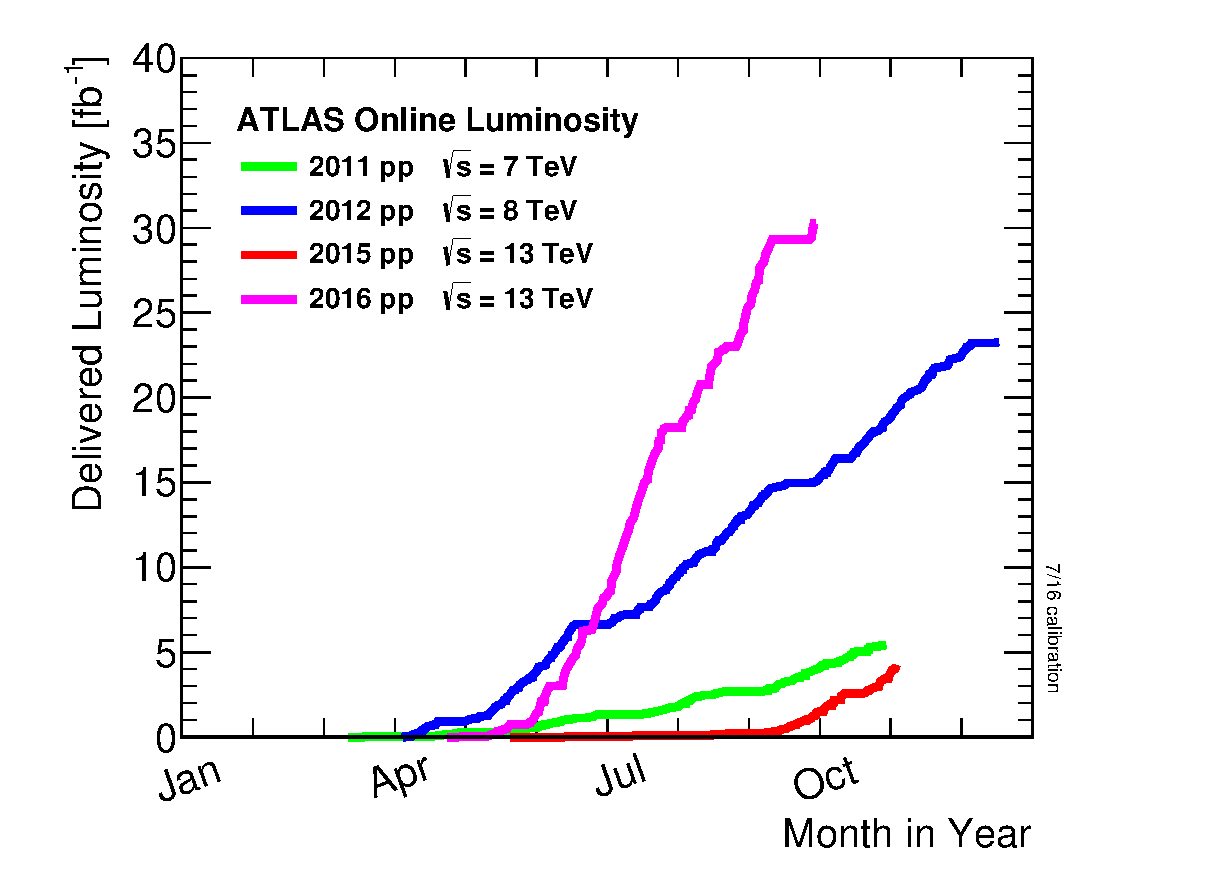
\includegraphics[width=.90\linewidth]{figures/lhc/intlumivsyear.eps}
\caption{ATLAS luminosity for Run 1 and Run 2, as of September 2016.}
\label{fig:lumi_vs_year}
\end{figure} 
\end{centering}

\section{Pile-up in proton-proton Collisions}
\label{sec:pileup}

One consequence of the high instantaneous luminosity is ``pile-up'', or multiple simultaneously interactions. Because each bunch has on order 100 billion protons, it is very likely that multiple protons will collide in the same bunch crossing. In fact, the average number of simultaneous interactions in 13 \tev data, shown in \autoref{fig:ninteractions}, is about twenty. 

\begin{centering}
\begin{figure}[!hbt]
\myfloatalign
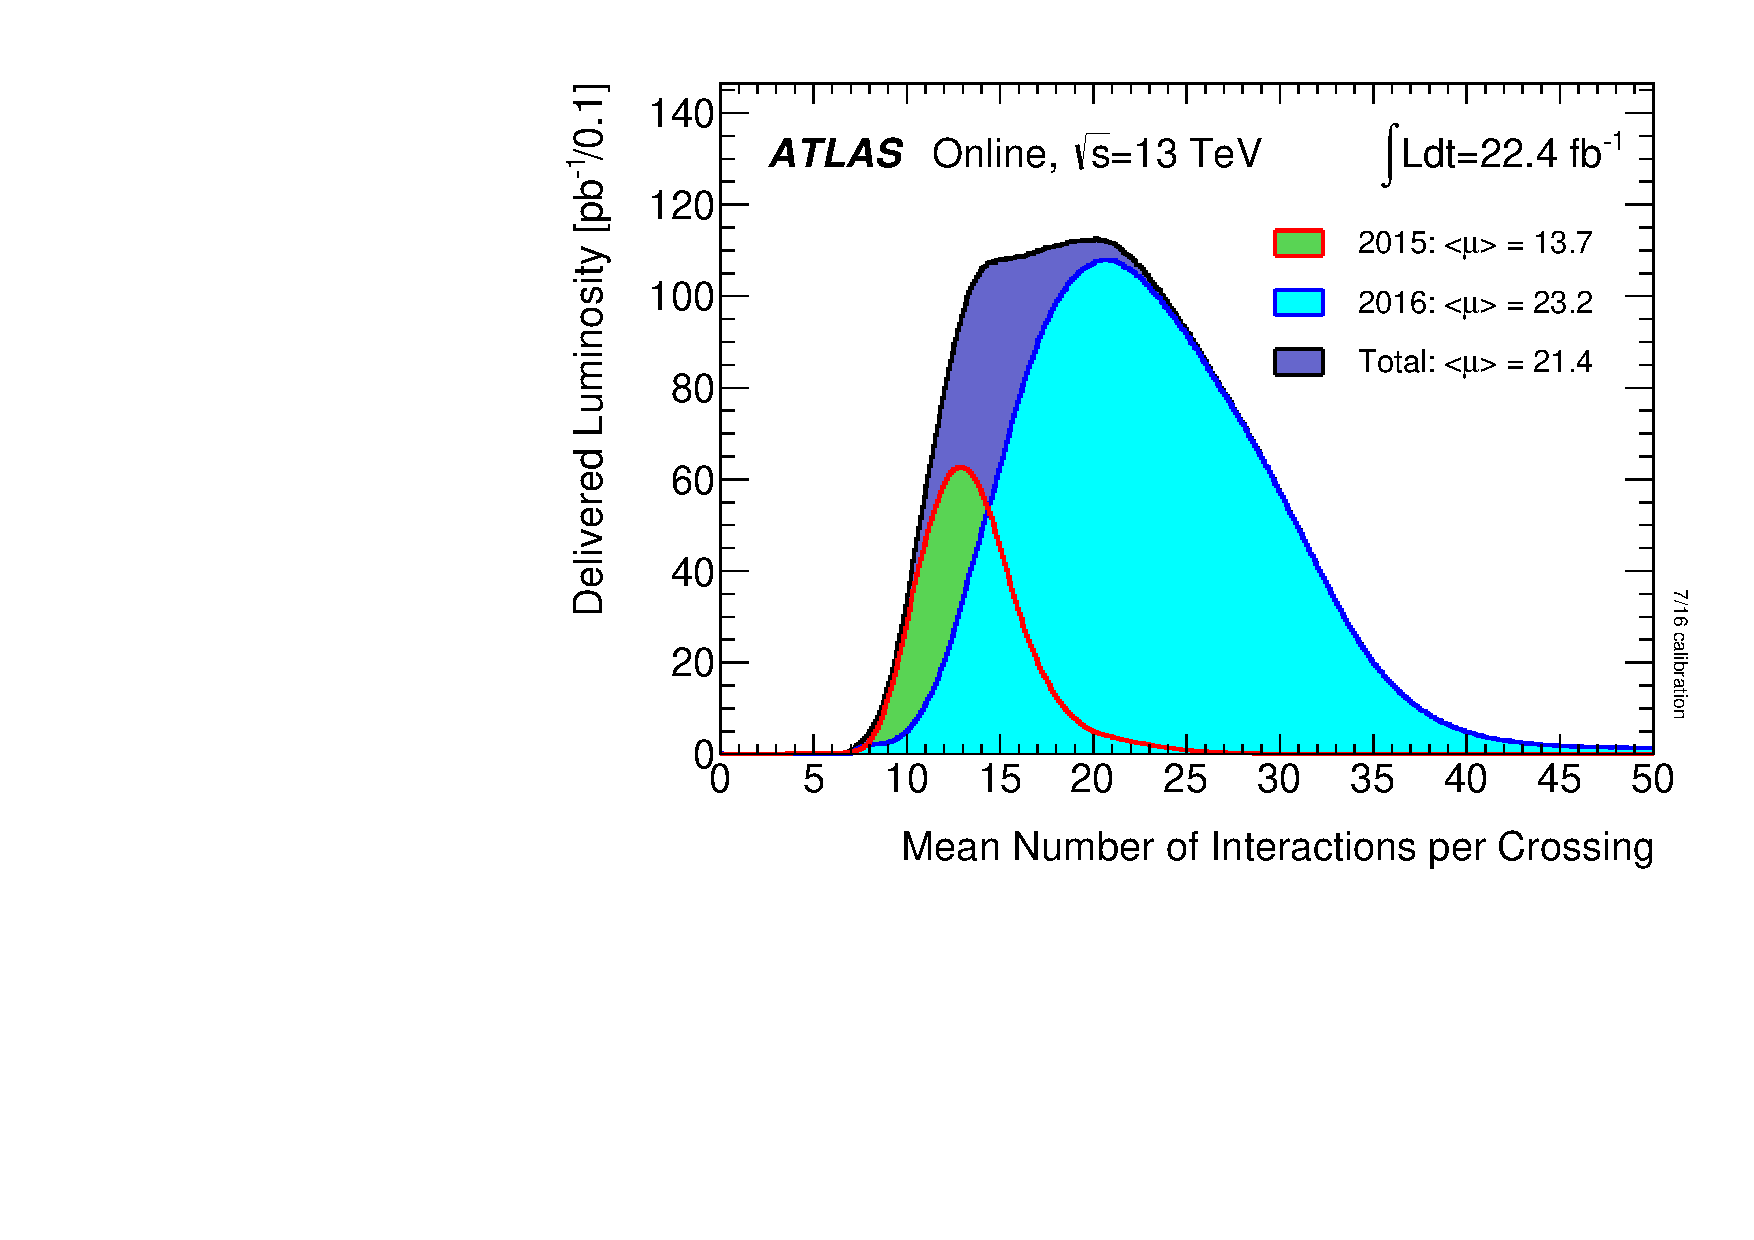
\includegraphics[width=.85\linewidth]{figures/atlas/mu_2015_2016_ICHEP.pdf}
\caption{Average number of interactions per crossing shown for 2015 and 2016 separately, as well as the sum of the two years.}
\label{fig:ninteractions}
\end{figure}
\end{centering}

Pile-up can be a difficult challenge for the ATLAS collaboration because it typically results in additional jets in an event, and can increase \ac{SM} backgrounds for analyses seeking to identify events with jets. It can also add to the overall hadronic energy of an event, and that energy can be mis-assigned to other objects. Fortunately, it is typically possible to resolve the different vertices that each proton-proton collision makes, and so pile-up jets can be identified and rejected. 


 % Chapter 3
%% Chapter X

\chapter{The ATLAS Detector} % Chapter title

\label{ch:atlas} % For referencing the chapter elsewhere, use \autoref{ch:name} 

The ATLAS detector circumscribes the \ac{LHC}'s beam pipe, enclosing the collision point with a series of particle detecting layers, aimed at making as many measurements of the particles leaving the collision point as possible. Its goal is to get a precise measurement of all the stable or semi-stable particles flying from proton-proton collisions at its center, allowing analyzers to fully reconstruct the kinematics of the underlying processes.

The ATLAS detector is the largest detector of its kind, measuring 44 m in length and 25 m in height, as seen in \autoref{fig:detector}. The size is mainly determined by the constraints of the \ac{MS}, discussed in \autoref{sec:MS}, which is the largest and outermost subsystem. The \ac{MS} is submerged in a spatially varying magnetic field provided by three toroidal magnets, while the \ac{ID} (\autoref{sec:ID}) is encased by a superconducting solenoid, which provides a uniform 2 T field throughout its volume \cite{PERF-2007-01}.

\begin{centering}
\begin{figure}[bth]
\myfloatalign
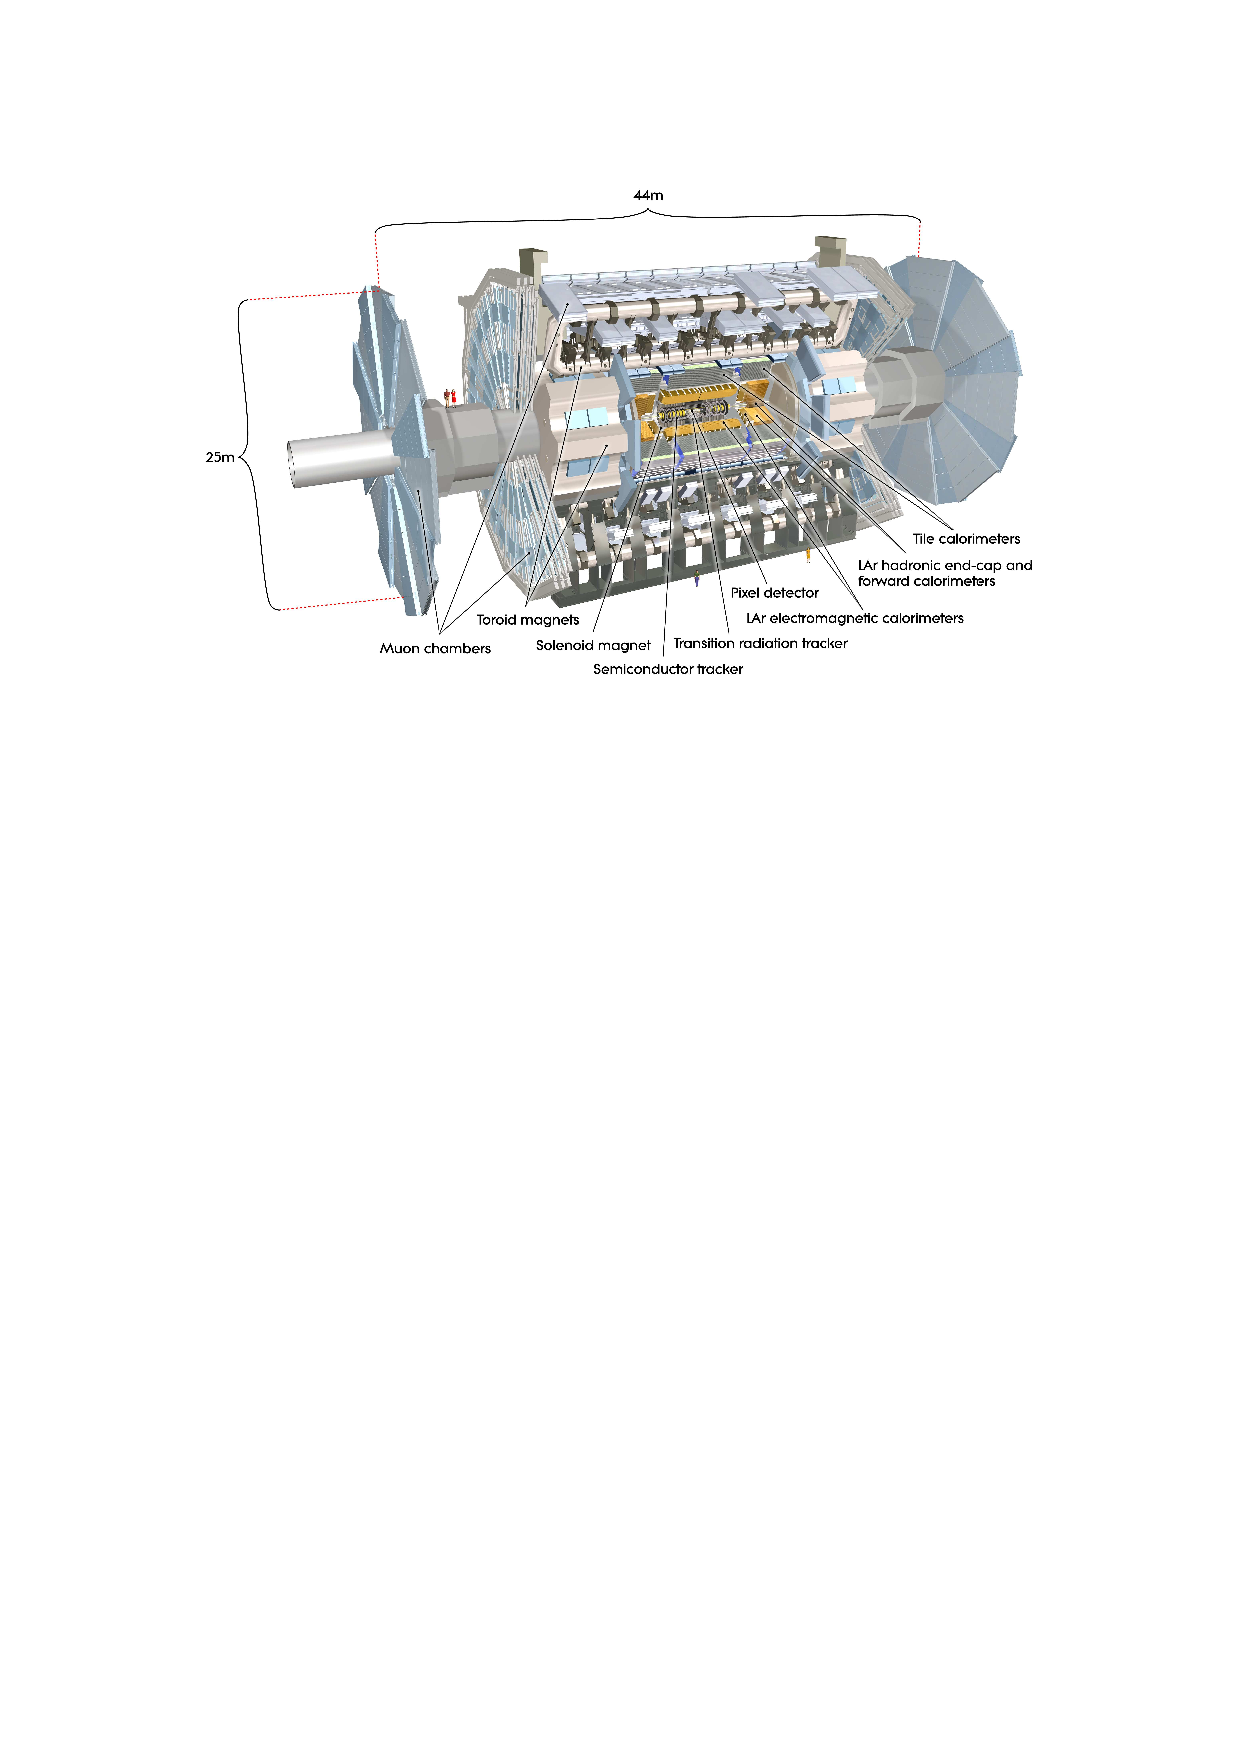
\includegraphics[width=.90\linewidth]{figures/atlas/detector.pdf}
\caption{Diagram of the ATLAS detector, with subsystems and magnets identified.}
\label{fig:detector}
\end{figure}
\end{centering}

\section{Coordinate System Used in the ATLAS Detector}

The ATLAS detector is centered around a the collision point in the beam pipe, and is built radially out from the pipe, maintaining as much rotational symmetry as possible. It is also symmetric in the forward-backward directions. Because of this geometry, a coordinate system using the collision point as the origin is used, with the beam pipe defining the $z$-axis. The positive $x$ direction is defined as pointing to the center of the \ac{LHC} ring, while the positive $y$ direction points upwards. For ease of reference, the side of the detector in the positive-$z$ direction is referred to as the A side, and the other side is referred to as the C side. 

Because of the radial design of the detector, angular coordinates are often used. The azimuthal angle $\phi$ defines the radial distance around the beam pipe and the polar angle $\theta$ defines the angle from the beam axis ($z$). However, a transformation of the polar angle called pseudorapidity ($\eta$) is used more often, and is defined as 

\begin{equation}
\eta = - ln [ tan \frac{\theta}{2} ]. 
\end{equation}

Building on this variable definition, distance between objects is typically defined as

\begin{equation}
\Delta R = \sqrt{\Delta\eta^2 + \Delta\phi^2}. 
\end{equation}

Often variables are defined purely in the transverse plane, which is indicated by a subscripted $T$, as in $p_T$, which gives an object's transverse momentum. Another common usage is $E_T^{miss}$, which gives the negative vectorial sum of the energy in an event. 

%------------------------------------------------

\section{The Inner Detector}
\label{sec:ID}

One goal of the ATLAS detector is to produce tracks, predictions of the paths particles take as they travel through the detector. Collisions in the detector produce about 1000 particles, so identifying and differentiating all these tracks is both a hardware and a computational challenge. The \ac{ID}, also called the Tracker, is responsible for providing high enough resolution measurements that each of these tracks and its precise position can be recorded. This tracking system consists of three subdetectors which each produce electrical responses to charged particles passing through their active material. Each of these signals is called a hit. ATLAS tracking software considers all these hits and forms tracks, with the goal of minimizing fake tracks due to random noise. Some details of this process is discussed at length in \autoref{sec:NN}. The full \ac{ID} can be seen in \autoref{fig:ID}, while a schematic in \autoref{fig:IDeta} demonstrates the $\eta$ coverage of each detector.

\begin{centering}
\begin{figure}[bth]
\myfloatalign
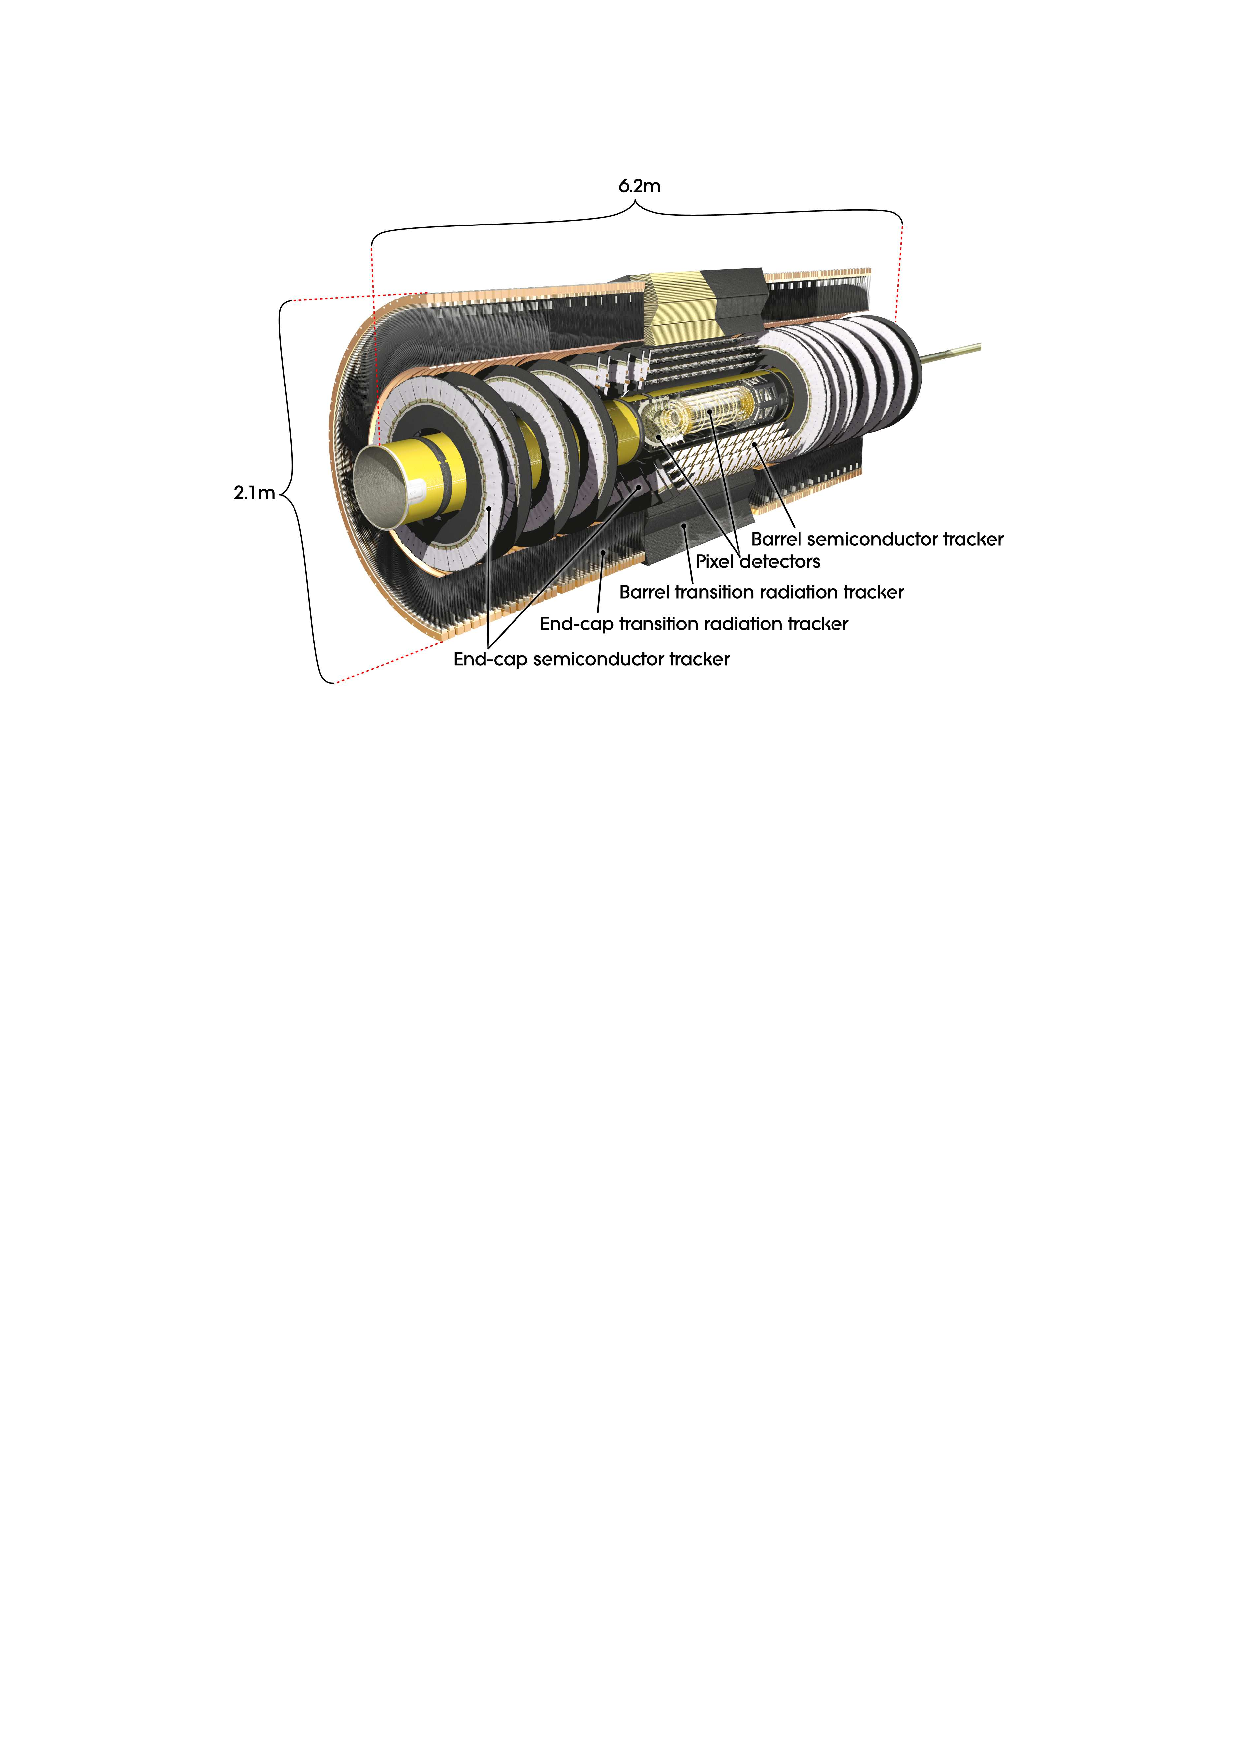
\includegraphics[width=.90\linewidth]{figures/atlas/innerdetector.pdf}
\caption{Diagram of the ATLAS Inner Detector, containing the Pixel, SCT, and TRT subsystems.}
\label{fig:ID}
\end{figure}
\end{centering}

\begin{centering}
\begin{figure}[bth]
\myfloatalign
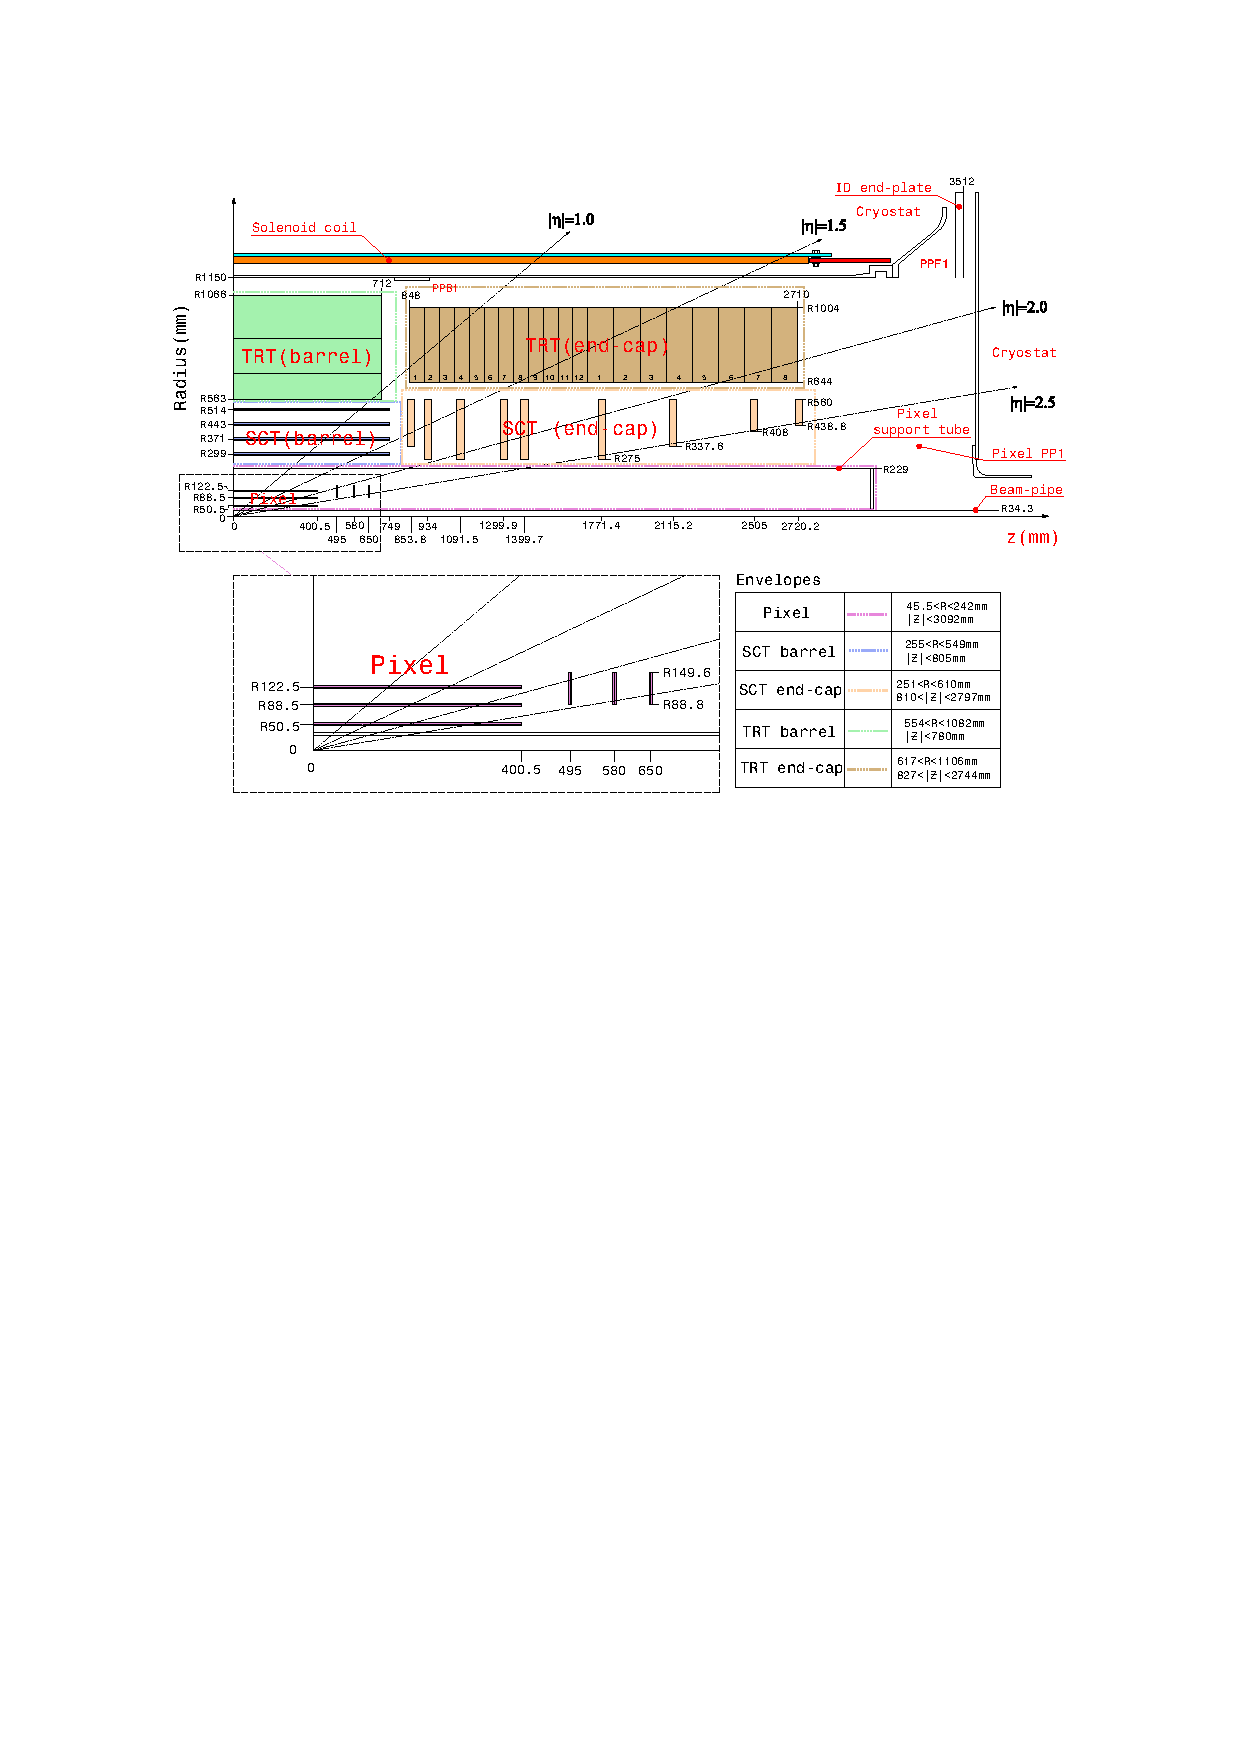
\includegraphics[width=.90\linewidth]{figures/atlas/ideta.pdf}
\caption{Diagram of one-quarter of the ATLAS Inner Detector, with lines drawn to indicate various $\eta$ locations. The labels PP1, PPB1 and PPF1 indicate the patch-panels for the ID services. TODO: what is that.}
\label{fig:IDeta}
\end{figure}
\end{centering}

\subsection{The Pixel Detector}

The Pixel detector lies closest to the beam pipe of the \ac{LHC}, and has four layers comprising 92 million read-out channels. There are three standard layers, referred to as Layers 1-3 (L1, L2, L3), and an additional layer added for the 2015 data-taking, called the \ac{IBL}. 

\subsubsection{The Original Pixel Detector}

The Pixel Detector consists of high-precision silicon chip pixel sensors, with 1744 sensors total. Each sensor is identical, containing 47232 pixels, which are typically each 50$\times$400 $\mu$m$^2$. 

As shown in \autoref{fig:IDeta}, the central $\eta$ region (barrel) is covered by three concentric cylindrical layers of sensors, while the higher $\eta$ region (endcap) is covered by a series of three disks positioned in the $x-y$ plane. Together, they give complete coverage out to $\eta = 2.5$, and a particle coming from the collision point will typically by measured by three layers. Each of these measurements is accurate in the barrel (endcap) to 10 $\mu$m in the $R-\phi$ direction and 115 $\mu$m in the $z$ ($R$) direction.  

\subsubsection{Addition of the IBL}

In 2015, the \ac{IBL} was lowered into the ATLAS cavern and added to the Pixel Detector. This layer sits on top of the beam pipe, inside barrel L1, which was formerly responsible for the first measurement of charged particles coming from a collision. 
TODO: add info about precision 


As the \ac{IBL}'s' name suggests, it was added to improve detection of $B$ mesons, whose non-trivial lifetimes create secondary vertices in ATLAS events, which allow them to be distinguished from other particles with precise track measurement. The \ac{IBL} is closer to the interaction point and has a smaller resolution, giving it a better chance to see these slightly displaced vertices.

\subsection{The Silicon Microstrip Tracker}

The \ac{SCT} employs similar technology to the Pixel Detector, with 15912 sensors and 6.3 million readout channels. Its difference from the Pixel Detector is in the readout, which is performed by a series of 12 cm long strips with a width of 80 $\mu$m. These layers are paired, placed on top of one another at a small (40 mrad) angle to allow for position determination in both directions, giving 4 spatial measurements for each particle passing through the \ac{SCT}. In the barrel, these strips run parallel to the beam pipe, while in the endcap, they are arranged radially. These strips have a resolution in the barrel (endcap) of 17 $\mu$m in the $R-\phi$ direction and 580 $\mu$m in the $z$ ($R$) direction. 

\subsection{The Transition Radiation Tracker}

The \ac{TRT} uses 4mm diameter gas-filled tubes, each with a high voltage wire suspended along the center of the tube. The tubes run the length of the barrel, with a separate wire in the positive and negative $z$ direction. In the endcap, the tubes are arranged radially. In total, there are about 351,000 readout channels in the \ac{TRT}. This detector makes measurements only in the $R-\phi$ direction, where the resolution of each measurement is 130 $\mu$m. Each particle typically creates about 36 hits as it passes through the \ac{TRT}. 

Particles passing through the gas mixture of the \ac{TRT} ionize the gas, producing electrons which drift towards the wire due to a potential difference applied between it and the straw. The \ac{TRT} also responds to low-energy transition radiation photons, which produce a much larger signal than charged particles passing through the detector. Because of this strong difference in signals, hits from the \ac{TRT} are used to help differentiate between electrons and photons in the detector.

\section{The Calorimeters}
\label{sec:Calo}

Unlike the tracking detectors, which aim to take measurements of a particle with minimal alterations of its trajectory, the calorimeters measure the the energy of objects by stopping them entirely. The calorimeters, which can be seen in \autoref{fig:calo}, provide coverage out to $\eta$ < 4.9. Higher granularity electromagnetic measurements are made within $|\eta|$ < 2.5, where the \ac{ID} provides tracking capability, in order to give precision measurements of the energy of photons and electrons, and provide reduced resolution measurements at higher $\eta$. The hadronic calorimeters provides coarser granularity, which is sufficient to determine the energy of jets. 

\begin{centering}
\begin{figure}[bth]
\myfloatalign
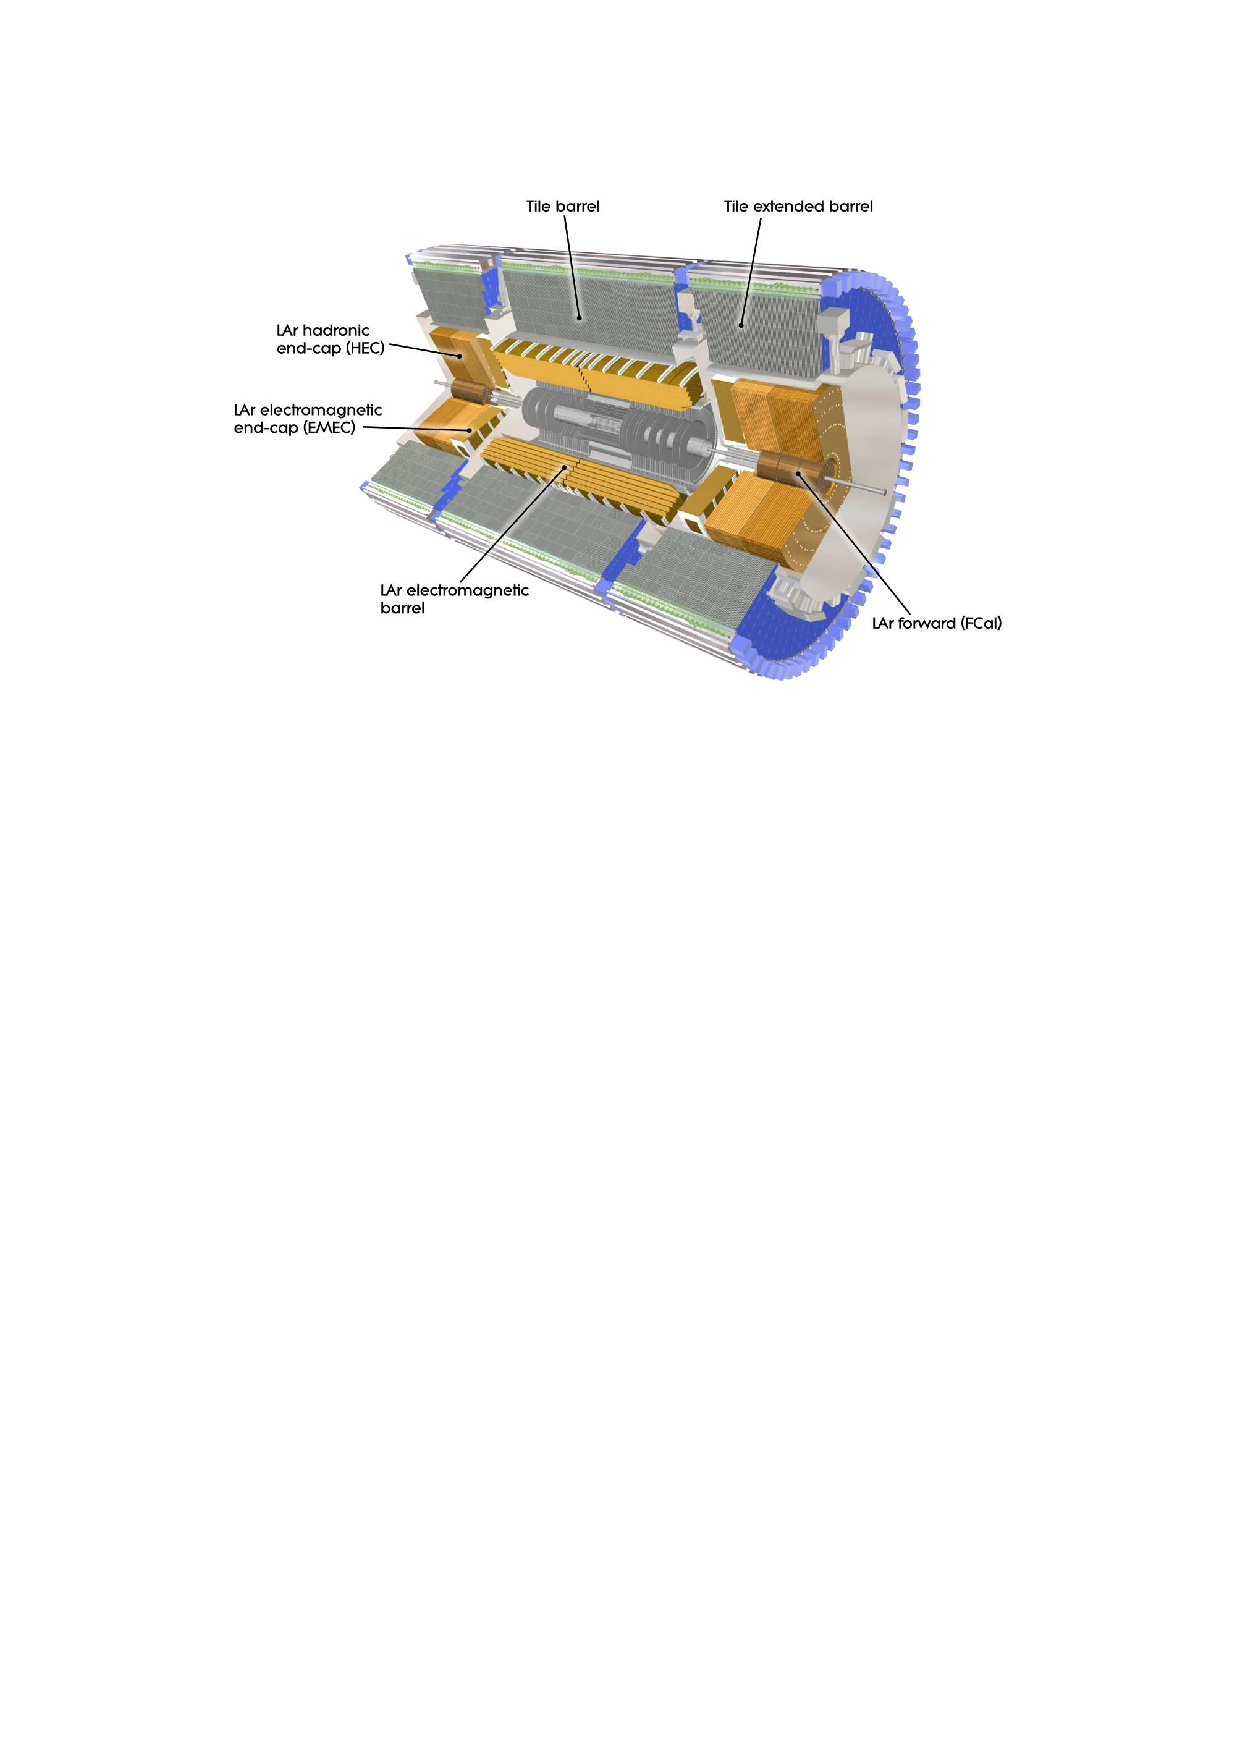
\includegraphics[width=.90\linewidth]{figures/atlas/calorimeters.pdf}
\caption{The calorimeter system of the ATLAS detector.}
\label{fig:calo}
\end{figure}
\end{centering}

%TODO make sure jets are in theory.

Another task of the calorimeter system is to limit punch-through to the \ac{MS}, described in \autoref{sec:MS}. All other particles must be fully stopped by the calorimeters to allow for clean signals from muons, and to measure the total energy of the particle. This requirement sets minimum sizes for each of the calorimeters. 

\paragraph{The LAr Electromagnetic Calorimeter} uses liquid argon as its active detector medium alternating with layers of lead acting as the absorber. The layers are shaped like accordions, which allows for complete coverage with multiple layers of active material, three in central $\eta$ ($0<|\eta|<2.5$) and two at higher $\eta$ ($2.5 < |\eta| < 3.2$). At $|\eta| < 1.8$, an instrumented liquid argon presampler provides a measurement of energy lost prior to reaching the calorimeters.

\paragraph{The Tile Calorimeter} is a hadronic calorimeter which surrounds the LAr Calorimeter. It uses layers of steel as its absorber with scintillating tiles as the active material between them, which are read out by photomultiplier tubes. The Tile Calorimeter covers $|\eta| < 1.7$. 

\paragraph{The LAr Hadronic Endcap Calorimeter} covers the hadronic calorimetery for higher $\eta$. It uses liquid argon active material and copper plate absorbers. This calorimeter covers $1.5 < |\eta| < 3.2$, overlapping with the hadronic calorimeters in either direction of its $\eta$ range. 

\paragraph{The FCal} or forward calorimeter provides electromagnetic and hadronic coverage at very high $\eta$ ($3.1 < |\eta| < 4.9$). This calorimeter also uses liquid argon as its active material, and uses copper-tungsten as the absorber. 

\section{The Muon Spectrometer}
\label{sec:MS}

The \ac{MS} measures charged particles that escape from the calorimeter system. Because the calorimeters are designed to completely absorb the energy of electrons, photons, hadrons, and jets, the \ac{MS} mainly detects muons, which escape from the calorimeter with very little loss of energy. The goal of the \ac{MS} is to give a high-precision measurement of these muons, and also to be able to quickly identify events with muons for the sake of triggering, discussed in \autoref{sec:Trigger}. The layout of the \ac{MS} can be seen in \autoref{fig:muon_xy} and \autoref{fig:muon_rz}. Muons can be measured for all $|\eta|$<2.7, and they can be triggered on for $|\eta|$<2.4. The entire system is about 24m tall and 40m long. 

\begin{centering}
\begin{figure}[bth]
\myfloatalign
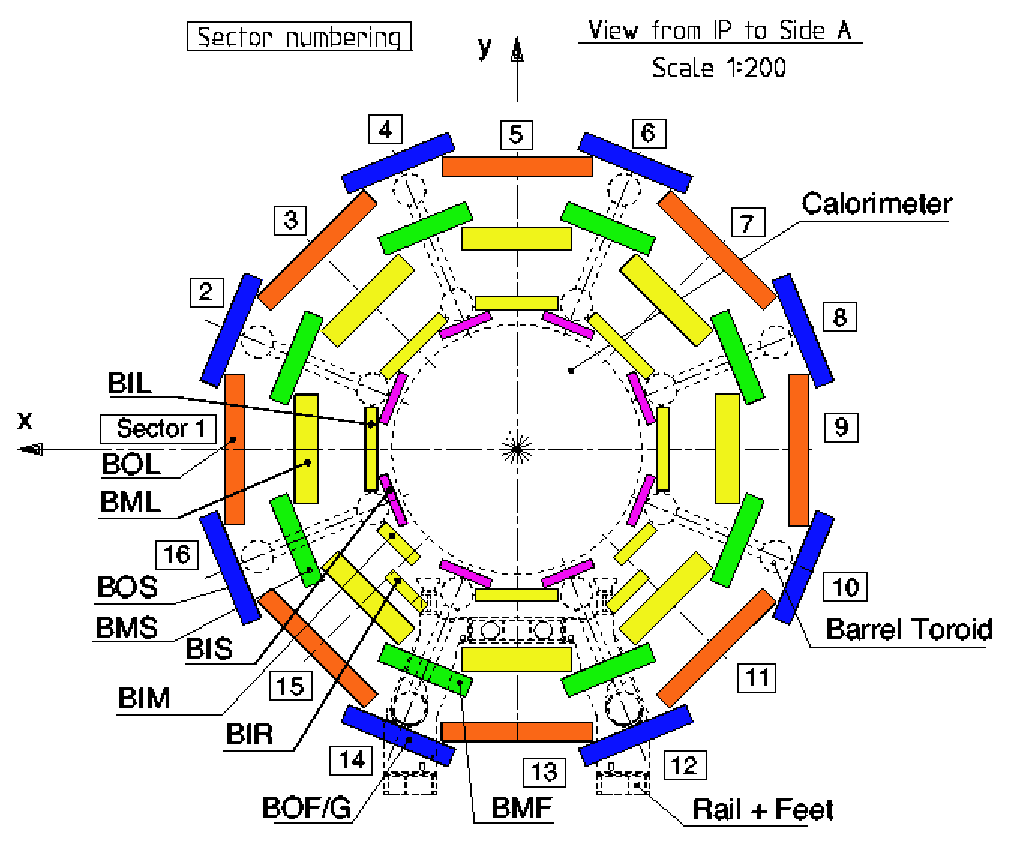
\includegraphics[width=.90\linewidth]{figures/atlas/Muon_sector_numbering.eps}
\caption{An $x$-$y$ view of the \ac{MS}. In it, the three barrel layers are visible, as well as the overlapping, differently sized chambers. The outer layer of the \ac{MS} is about 20m in diameter.}
\label{fig:muon_xy}
\end{figure}
\end{centering}

\begin{centering}
\begin{figure}[bth]
\myfloatalign
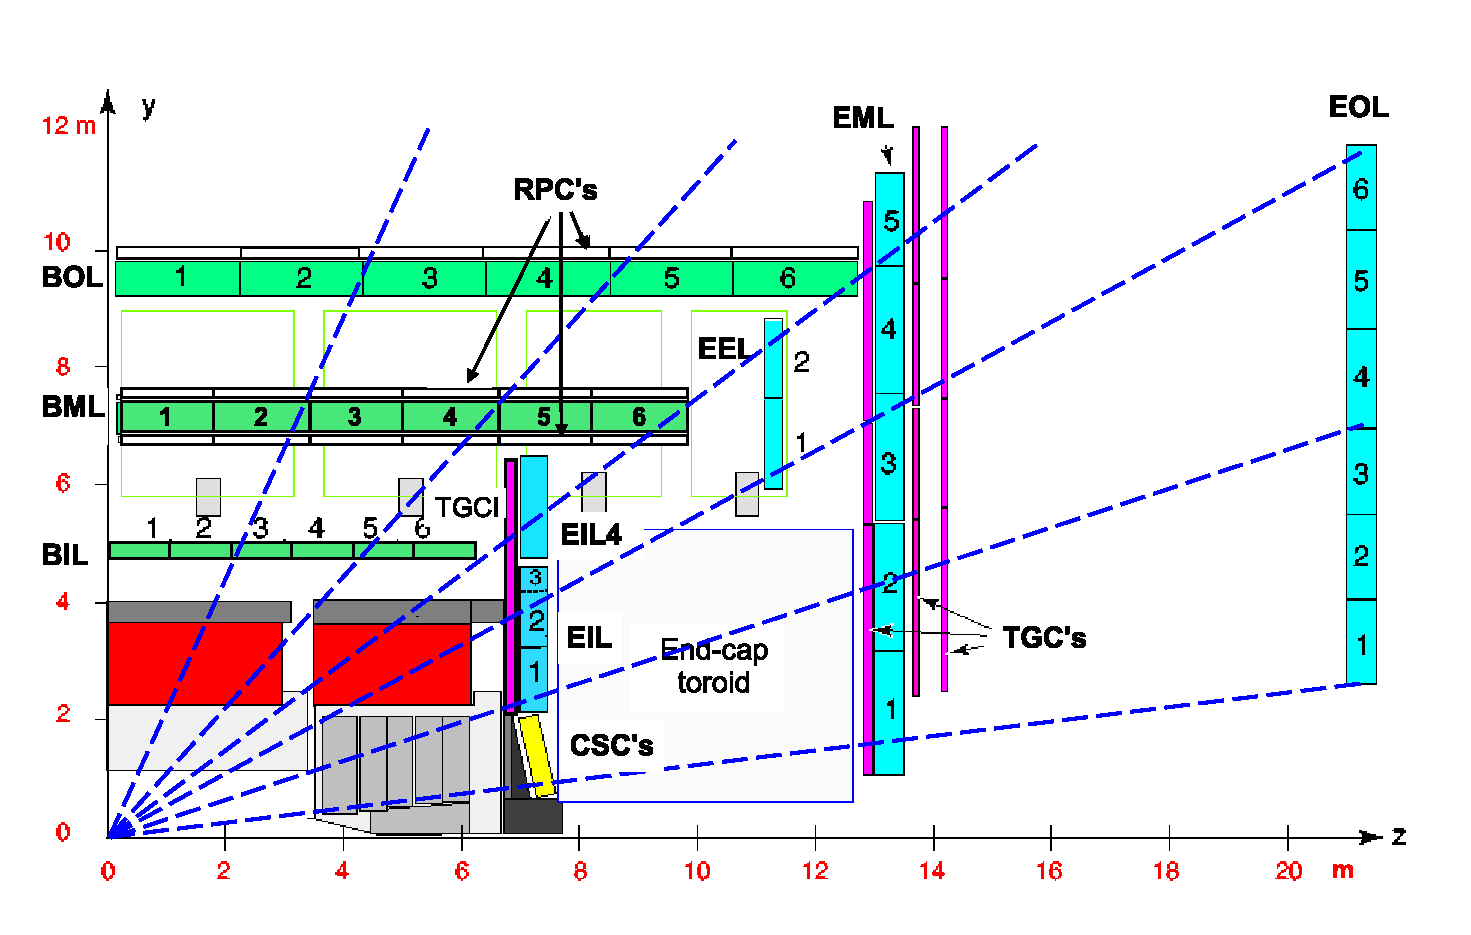
\includegraphics[width=.90\linewidth]{figures/atlas/Muon_rz_large_sect_6.eps}
\caption{An $r$-$z$ view of the \ac{MS}. The three layers of the barrel and endcap \ac{MS} are visible, and all muons at $|\eta|$<2.7 should traverse three detectors, assuming they propagate in an approximately straight line from the interaction point.}
\label{fig:muon_rz}
\end{figure}
\end{centering}

To achieve these goals, the \ac{MS} has several subsystems. The system responsible for precision measurement is called the \acp{MDT}. This subdetector consists of chambers of three to eight layers of tubes, with three layers of chambers covering both the barrel and end-cap regions. The tubes each contain an Ar/CO$_2$ gas mixture and a single high voltage wire which runs at its center along its length. Charged particles excite the gas as they pass through it, producing electrons which drift towards the high voltage wire. The resulting electric signal is read out, and the magnitude and timing of the signals are both used to differentiate particle traces from noise. 

Though very effective at giving a precise measurement, the \acp{MDT} have several shortcomings. The first is that the measurement is only precise in the direction perpendicular to the tubes; in the direction parallel to them, the resolution is not much better than the length of the drift tube. The resolution in the perpendicular direction is about 35 $\mu$m with the combined measurement of all the tubes in a chamber. 

The \acp{MDT} are slow, with a maximum drift time of about 700ns. Because collisions occur every 25ns, this readout cannot be used for triggering. In addition, in high-rate regions of the detector, the \acp{MDT} are very susceptible to having multiple hits in one readout window. To minimize this effect, another detector called the \acp{CSC} is used. This detector consists of multi-wire proportional chambers which have cathode strips on either side of the anode in orthogonal directions, allowing for a 40$\mu$m resolution in one direction and 5mm resolution in the other. Their drift times are also much faster than the \acp{MDT}, at about 40ns, so they are placed in the forward region of the detector (2<$|\eta|$<2.7) where the incident particle rates are much higher. 

To achieve rates fast enough to be used for triggering, the \acp{RPC} and \acp{TGC} are used. These chambers can produce track information roughly as fast as the collision rate. The \acp{RPC} are used in the barrel and are made up of two high-resistance plastic plates with a gas mixture under an electric field between them. Passing particles ionize this gas, and the resulting signal is read out via metallic strips mounted to the plastic plates. The \acp{TGC} used in the endcap are a form of multi-wire proportional chambers, like the \acp{CSC}. Unlike the \acp{CSC}, the cathode is placed extremely close to the wires, speeding up its operation. 

The massive system is also subject to deformations due to gravity. To maintain this good precision, these deformations are constantly monitored in each chamber with a set of four optical alignment rays, which give alignment information at the precision of <30$\mu$m. In addition, a sag-adjustment system can use this information to re-align any wires that droop under gravity's pull. Lastly, the \ac{MS} can be aligned using the tracks made from hits it measures, discussed more in \autoref{sec:reco_muons}.

\section{The Magnet System}
\label{sec:magnets}

The ATLAS magnet system consists of four superconducting magnets: an inner solenoid, a barrel toroid, and two endcap toroids. Collectively, they are 22m in diameter and 26m long, and their basic layout can be seen in \autoref{fig:magnets}.

\begin{centering}
\begin{figure}[bth]
\myfloatalign
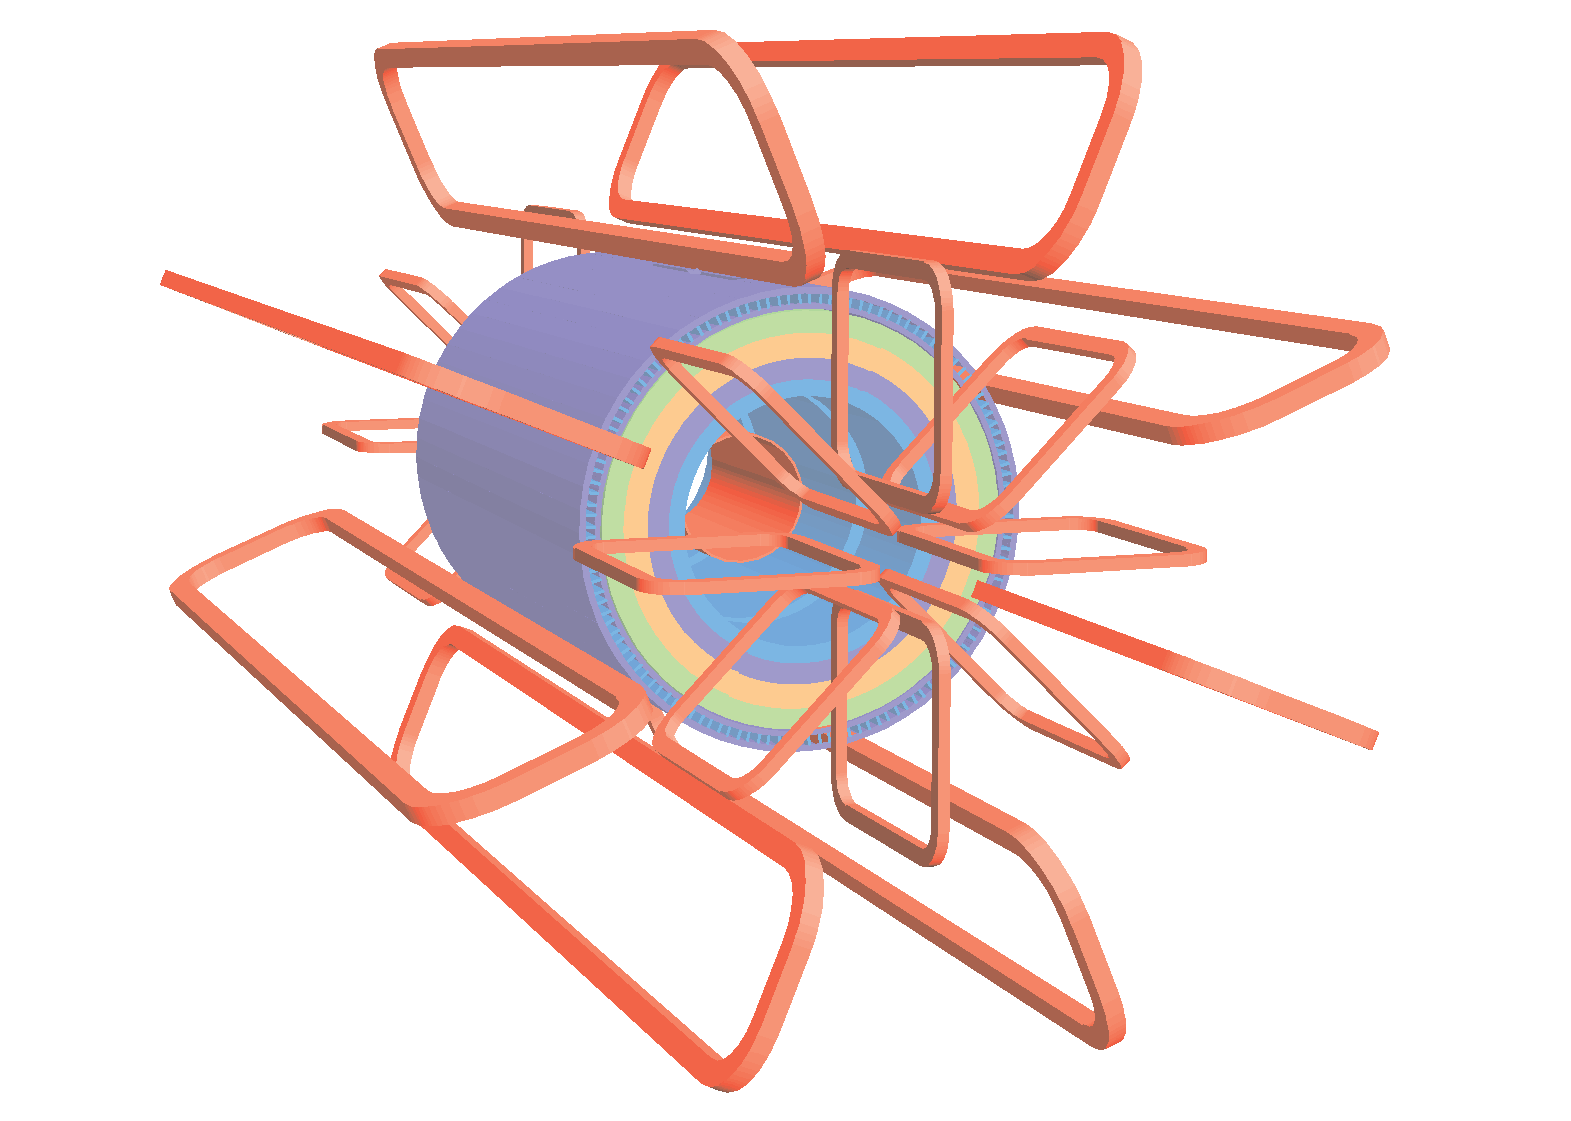
\includegraphics[width=.90\linewidth]{figures/atlas/ATLcoilGeom.eps}
\caption{The magnet system of the ATLAS detector. The inner cylinder shows the solenoid which gives a uniform magnetic field in the \ac{ID}. Outside of that are the barrel and endcap toroids, which provide a non-uniform magnetic field for the \ac{MS}.}
\label{fig:magnets}
\end{figure}
\end{centering}

The solenoid sits inside the calorimeter volume and provides a uniform 2T magnetic field to particles traveling through the \ac{ID}. This axial field causes the trajectories of charged particles to bend in the $x-y$ plane, and measurements of the curvature of these trajectories give the most accurate \pt measurement for many particles. 

Because the solenoid sits between the tracking system and the calorimeter, it is important that it interfere minimally with particles in order to allow the calorimeter to measure their full energies. The solenoid is placed inside the same vacuum chamber as the LAr calorimeter and is made of Al-stabilized NbTi superconductor with aluminum casing, giving it a total thickness of about 0.66 radiation lengths. 

The barrel toroid sits outside the calorimeters and provides the magnetic field for the barrel \ac{MS}, which varies from 0.2–2.5T. The endcap toroids have a magnetic field range of 0.2-3.5T. All three toroid magnets are made with Al-stabilized Nb/Ti/Cu superconducting coils supported by Al-alloy struts. 

The magnets are cooled with liquid helium, and take up to a month to be brought down to operating temperatures. All magnets have cold masses surrounding them to absorb heat in the event of a quench. 

The $B$-field resulting from this magnet system can be seen in \autoref{fig:bfield}. The plot on the left demonstrates the relatively constant field rate within the barrel which drops steeply at $|z|$=2. The right plot shows the field integral in the \acp{MDT} as a function of $|\eta|$, demonstrating the good coverage out to $|\eta|$<2.6 excluding a transition region between the barrel and endcap, where the field can can drop to around half its usual value. 

\begin{centering}
\begin{figure}[bth]
\myfloatalign
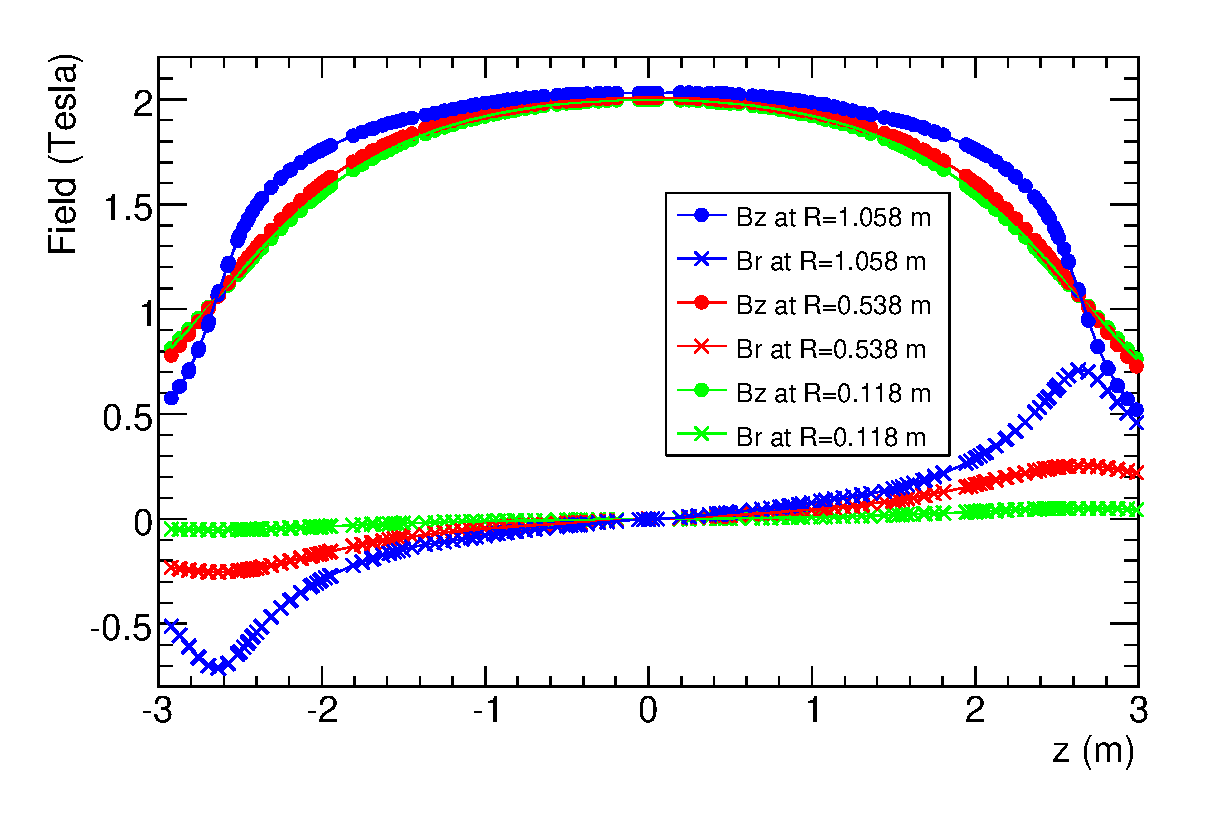
\includegraphics[width=.45\linewidth]{figures/atlas/solMeasB.eps}
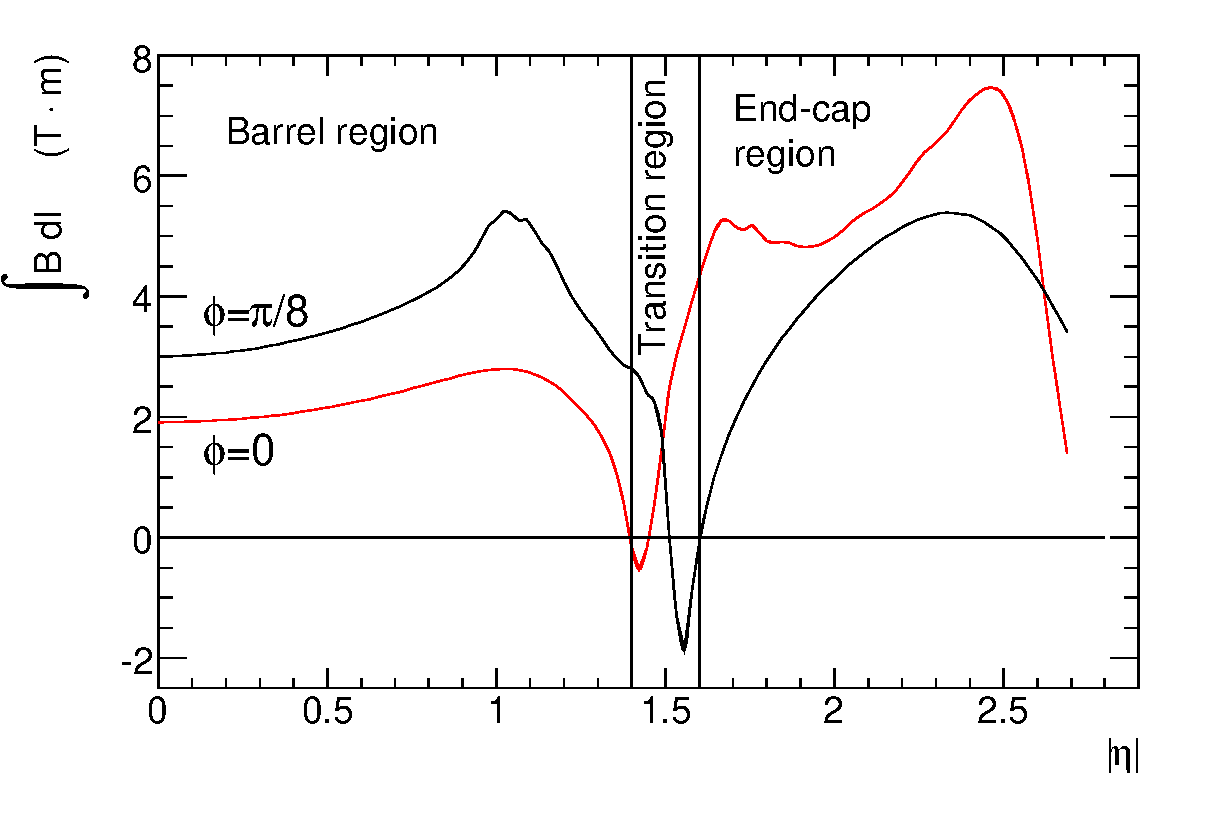
\includegraphics[width=.45\linewidth]{figures/atlas/IBdl.eps}
\caption{Plots of the magnetic field within the ATLAS detector. Left is the field (broken into its $R$ and $z$ components) as a function of $z$ for several different values of $R$. Right is the field integral through the \acp{MDT} as a function of $|\eta|$ for two different $\phi$ values. }
\label{fig:bfield}
\end{figure}
\end{centering}

\section{The Trigger System}
\label{sec:Trigger}

The \ac{LHC} provides proton bunch crossings every 25ns, and each of these events contains about one Mb of data, corresponding to 40Tb/s, a completely unmanageable amount of data. In addition to this concern, many of ATLAS's subdetectors like the pixel detector and \acp{MDT} take much longer than 25ns to read out, making keeping up with the bunch crossing rate impossible. To reduce the total data read out and allow for selective reading out of the slower detectors, a triggering system is used. 

The trigger system uses fast detectors to get a coarse picture of an event's topology, which is then compared to a trigger menu, which lists the types of events that are interesting enough to keep. Overall, the trigger system reduces the 40 million collisions a second to about 1000 to be fully read out from the ATLAS detector. 

This filtering of events is done in two steps: the \ac{L1} trigger is implemented in hardware and reduces the initial 40MHz to 100kHz, while the \ac{HLT} is implemented in software, further reducing the rate to 1kHz \cite{ATL-DAQ-PUB-2016-001}.The \ac{L1} trigger uses coarse granularity information from the fast read-out subdetectors: the calorimeters, the \acp{RPC} and \acp{TGC}. 

The coarse grained calorimeter information used for the \ac{L1} trigger decision is referred to as \ac{L1Calo} and uses information from all calorimeter systems. \ac{L1Calo} is responsible for all triggers excluding muons, meaning it must be capable of identifying a large number of different objects and event topologies, including high-\pt objects, large amounts of \met, andlarge amounts of hadronic energy.  
The outputs from the different calorimeters and the \ac{MS} can also be combined with a system called \ac{L1Topo}. Using this, triggers can require more complex topologies, and can suppress backgrounds from pileup by rejecting  


 % Chapter 4 - empty template

\cleardoublepage % Empty page before the start of the next part

%----------------------------------------------------------------------------------------
%	THESIS CONTENT - APPENDICES
%----------------------------------------------------------------------------------------

\appendix

\part{Appendix} % New part of the thesis for the appendix

% Appendix A

\chapter{Appendix Test}

%----------------------------------------------------------------------------------------

\lipsum[13-14]

%----------------------------------------------------------------------------------------

\section{Appendix Section Test}
\lipsum[15]

\graffito{More dummy text}
\lipsum[16]

%----------------------------------------------------------------------------------------

\section{Another Appendix Section Test}
\lipsum[17]

\begin{table}
\myfloatalign
\begin{tabularx}{\textwidth}{Xll} \toprule
\tableheadline{labitur bonorum pri no} & \tableheadline{que vista}
& \tableheadline{human} \\ \midrule
fastidii ea ius & germano &  demonstratea \\
suscipit instructior & titulo & personas \\
\midrule
quaestio philosophia & facto & demonstrated \\
\bottomrule
\end{tabularx}
\caption[Autem usu id]{Autem usu id.}
\label{tab:moreexample}
\end{table}

\lipsum[18]

There is also a useless Pascal listing below: \autoref{lst:useless}.

\begin{lstlisting}[float=b,language=Pascal,frame=tb,caption={A floating example (\texttt{listings} manual)},label=lst:useless]
for i:=maxint downto 0 do
begin
{ do nothing }
end;
\end{lstlisting} % Appendix A
%% Appendix X

\chapter{Appendix Title}

%----------------------------------------------------------------------------------------

% Content begins here % Appendix B - empty template

%----------------------------------------------------------------------------------------
%	POST-CONTENT THESIS PAGES
%----------------------------------------------------------------------------------------

\cleardoublepage% Bibliography

\label{app:bibliography} % Reference the bibliography elsewhere with \autoref{app:bibliography}

\manualmark % Work-around to have small caps also here in the headline
\markboth{\spacedlowsmallcaps{\bibname}}{\spacedlowsmallcaps{\bibname}} % Work-around to have small caps also
%\phantomsection
\refstepcounter{dummy}

\addtocontents{toc}{\protect\vspace{\beforebibskip}} % Place the bibliography slightly below the rest of the document content in the table of contents
\addcontentsline{toc}{chapter}{\tocEntry{\bibname}}

\printbibliography % Bibliography

\cleardoublepage% Declaration

\refstepcounter{dummy}
\pdfbookmark[0]{Declaration}{declaration} % Bookmark name visible in a PDF viewer

\chapter*{Declaration} % Declaration section text

\thispagestyle{empty}

Put your declaration here.
\bigskip
 
\noindent\textit{\myLocation, \myTime}

\smallskip

\begin{flushright}
\begin{tabular}{m{5cm}}
\\ \hline
\centering\myName \\
\end{tabular}
\end{flushright}
 % Declaration

\cleardoublepage% Colophon (a brief description of publication or production notes relevant to the edition)

\pagestyle{empty}

\hfill

\vfill

\pdfbookmark[0]{Colophon}{colophon}

\section*{Colophon}

This document was typeset using the typographical look-and-feel \texttt{classicthesis} developed by Andr\'e Miede. The style was inspired by Robert Bringhurst's seminal book on typography ``\emph{The Elements of Typographic Style}''. \texttt{classicthesis} is available for both \LaTeX\ and \mLyX: 

\begin{center}
\url{https://bitbucket.org/amiede/classicthesis/}
\end{center}

\noindent Happy users of \texttt{classicthesis} usually send a real postcard to the author, a collection of postcards received so far is featured here: 

\begin{center}
\url{http://postcards.miede.de/}
\end{center}
 
\bigskip

\noindent\finalVersionString % Colophon

%----------------------------------------------------------------------------------------

\end{document}
